% Ab hier arabische Seitenzählung und heading Seitenstil
\pagestyle{scrheadings}
\pagenumbering{arabic}

\chapter{Einleitung}
- ganz am Ende

\chapter{System- und Problembeschreibung}

\section{Demonstratorsytem}
Im Rahmen vorangegangener studentischer Arbeiten ist am Fraunhofer-Institut für Integrierte Schaltungen IIS, Institutsteil Entwicklung Adaptiver Systeme EAS \cite{fraunhoferIISEAS} in Dresden ein Demonstratorsystem entwickelt worden. Langfristig soll dieses Vorteile von Regelungsstrategien auf verteilten Recheneinheiten gegenüber einer zentralen Messgrößenverarbeitung und Stellgrößenberechnung untersuchen. Der Demonstrator ist in Abbildung \ref{fig:demonstrator_real} dargestellt.

\begin{figure}[ht]
	\begin{center}
		% hier keine Skalierung notwendig, wenn Datei schon mit passender figsize angelegt wurde:
		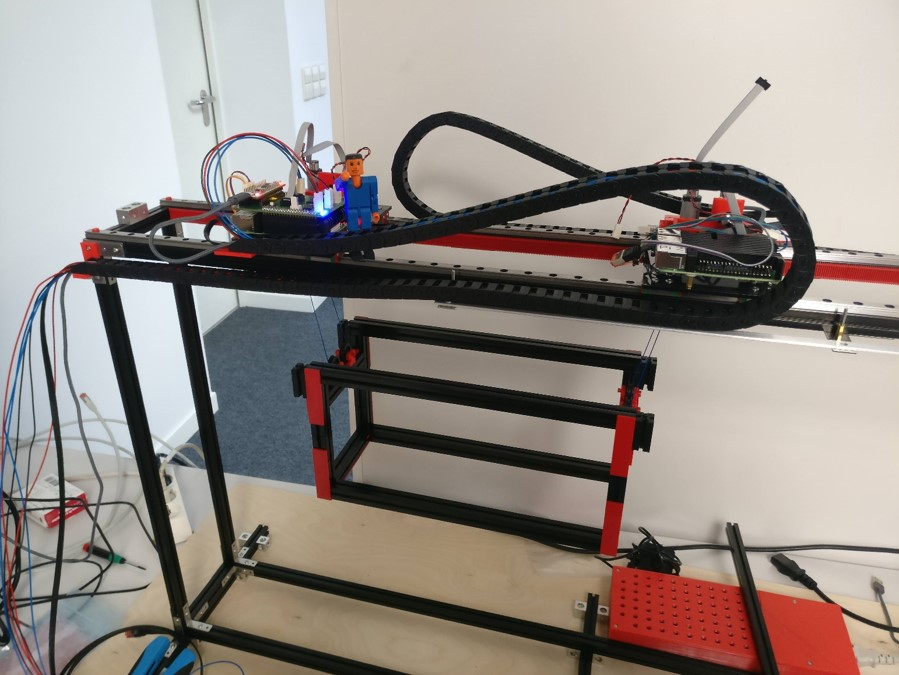
\includegraphics[scale=1]{Pictures/real_gantry.jpg}
	\end{center}
	\caption[Doppelkran-Demonstratorsystem mit Laufkatzen und Last]
	{Doppelkran-Demonstratorsystem mit Laufkatzen und Last.}
	\label{fig:demonstrator_real}
\end{figure}

Das Demonstratorsystems besteht aus zwei Brückenkränen, die eine gemeinsame Last in einer festen Ebene anheben. Die Kräne befinden sich auf Schienen und verfügen jeweils über einen Raspberry Pi 4B als Hauptrecheneinheit sowie einen STM32-Mikrocontroller für Motoransteuerungen und Messungen. Beide Raspberry Pis können über eine LAN-Verbindung miteinander kommunizieren.

Beide Kräne sind auf Schienen in horizontaler Richtung sowie die Seillängen mit jeweils einem DC-Motor aktuiert. Auf den STM32-Mikrocontroller ist bereits eine eine unterlagerte Strom- beziehungsweise Kraftregelung für diese implementiert.
Messungen der Seillängen und Kranpositionen auf der Schiene erfolgen mittels Inkrementalgebern nach einem anfänglichen Kalibrierungsvorgang. Die Seilwinkel werden mittels mitschwingender Potentiometer bestimmt.




\section{Problembeschreibung und Zielsetzung}
Bei der Bewegung von Containern in Häfen ist ein ruckarmer und gegenüber der Horizontalen stabiler Transport notwendig. Ziel der Studienarbeit ist es deshalb,  bezüglich des vorhandenen Demonstratorsystems eine zentrale Referenzregelstrategie zu entwerfen. Damit soll unter Vorgabe von Sollposen eine Planung von Trajektorien der Last in der Ebene und Folgeregelung zur Überführung dieser zwischen verschiedenen Ruhelagen ermöglicht werden. Diese Überlegungen sollen auf Basis einer Modellierung des Krans als Mehrkörpersystems geschehen. 

\chapter{Analytische Modellbildung}

\section{Allgemeine Modellannahmen}

In der folgenden Modellierung wird das Demonstratorsystem nur planar betrachtet, also die gesamte Bewegung aller Komponenten nur in der vertikalen Ebene berücksichtigt. Diese Annahme ist gerechtfertigt, weil die Laufkatzen nur entlang einer Achse verfahren können und die Lagerung bzw. Aufhängung der Last ein Schwingen dieser nur in einer Ebene zulässt. Die Seile werden aufgrund der geringen Dicke und auch im Vergleich zu den Laufkatzen und der Last als masselos angenommen sowie nicht mit einem Trägheitsmoment behaftet. Die Last wird trotz ihrer Aussparungen mit einer homogenen Masseverteilung modelliert. Für eine exakte Beschreibung wären CAD-Daten oder eine Demontage mit Vermessung der Teilkomponenten notwendig. Es wird aus Gründen der Einfachheit auf die Abbildung dissipativer Kräfte verzichtet. Zudem können diese bei einer funktionierenden unterlagerten Regelung als kompensiert angenommen werden.

Die Modellbildung erfolgt in mehreren Stufen. Es ist zunächst problemlos möglich mittels der Lagrange-Gleichungen erster oder auch zweiter Art den Einzelkran darzustellen. Dabei hat die Modellierung zweiter Art den Vorteil, dass Stellkräfte einfacher abgebildet werden können und sich ein typischerweise effizient zu simulierendes gewöhnliches Differenzialgleichungssystem (DGL-System, engl. ODE systems) ergibt. Ausgehend von den Erkenntnissen und aufgrund geringer Komplexität der überschaubaren Terme des Einzelkrans, kann die prinzipielle Methodik verifiziert werden. Daran anschließend wird eine Erweiterung auf ein Doppelkransystem in Analogie zum realen Demonstrator vorgenommen. Wegen der an beiden Laufkatzen befestigten Last liegt zunächst alternativ zum vorherigen Vorgehen die Nutzung der Lagrange-Gleichungen erster Art, bei der mittels algebraischer Zwangsbedingungen ein Differenzial-algebraisches Gleichungssystem (DAE-System, von engl. differential algebraic equations) zur Simulation generiert wird, nahe. Allerdings ist dabei eine Aktuierung der Seilwinden anspruchsvoller, da bereits für eine konstante Seillänge die bei der Katzfahrt auftretenden dynamischen Seilkräfte kompensiert werden müssen, ohne dass es dafür eine explizite resultierende Gesamtkraft gibt, die zu Null gesetzt werden kann. Beim physischen Demonstrator sperrt das Schneckengetriebe der Seilwinde im stromfreien Fall die Hubaktuierung. Auch bei einem Doppelkransystem ist stattdessen eine Modellierung mit den Lagrange-Gleichungen zweiter Art möglich. Es folgt nun eine kurzer theoretischer Überblick zu beiden erwähnten Arten des Lagrange-Formalismus.

\section{Modellierung mittels Lagrange-Formalismus}

Eine stark automatisierte Durchführung dieses Formalismus ist unter Nutzung des Python-Pakets symbtools \cite{symbtools} möglich.

\subsection{Lagrange-Gleichungen erster Art}
\label{sec:Lagrange1_theory}
Die Dynamik mechanischer Systeme lässt sich über Differenzialgleichungen, den so genannten Lagrange-Gleichungen beschreiben. Dabei wird eine Menge aus $n$ auftretenden und zeitlich veränderlichen Koordinaten als Konfigurationskoordinaten oder Systemgrößen $\mathbf{\theta} = (\theta_1, ..., \theta_n)^T$ bezeichnet. Die zeitlichen Änderungsraten dieser sind die (Konfigurations-)Geschwindigkeiten $\dot{\mathbf{\theta}}$ \cite[S.7]{DissKnoll}. 

Die kinetische Energie eines Systems wird im Folgenden durch die Funktion $T$ sowie die potentielle Energie durch $V$ beschrieben. Die Lagrange-Funktion kann damit folgendermaßen definiert werden:
\begin{equation}
	L(\mathbf{\theta}, \dot{\mathbf{\theta}}) = T(\mathbf{\theta}, \dot{\mathbf{\theta}}) - V(\mathbf{\theta}).
\end{equation}

Mit den Lagrange-Gleichungen erster Art können Probleme mit Zwangsbedingungen und -kräften dargestellt werden:
\begin{equation}
	\diff{}{t}\left(\partiell{L}{\dot{\theta}_i} \right) - \partiell{L}{\theta_i} = \tilde{Q}_i + Q_i, \quad i = 1, ..., n.
\end{equation}

Die sich auf die jeweilige Koordinate $\theta_i$ beziehende Stellkraft $Q_i = f_i - D_i$ entspricht der verallgemeinerten Kraft, welche sich aus der äußeren (Stell-)Kraft $f_i$ sowie internen Reibungskraft $D_i$ zusammensetzt \cite[S. 49]{Lagrange}.

Es können $m$ holonomen Zwangsbedingungen $g_1(\mathbf{\theta}) = ... = g_m(\mathbf{\theta}) = 0$ eingeführt werden, aus denen die Zwangskraft $\tilde{Q}_i$ in Richtung der Koordinate $\theta_i$ folgt:
\begin{equation}
	\tilde{Q}_i = \sum_{j = 1}^m \lambda_j \left(\partiell{g_j}{\mathbf{\theta}}\right)^T.
\end{equation}
In dieser Beziehung bezeichnet $\lambda_j$ den jeweiligen Lagrange-Multiplikator.

\subsection{Lagrange-Gleichungen zweiter Art}
\label{sec:Lagrange2_theory}
Die Lagrange-Gleichungen zweiter Art beschreiben bezüglich des Vorhergehenden den Spezialfall ohne Zwangsbedingungen, also $m = 0$. Zwangskräfte müssen dabei nicht explizit bestimmt werden. Die Bewegungsgleichungen können folgendermaßen aus der Lagrange-Funktion abgeleitet werden:
\begin{equation}
	\diff{}{t}\left(\partiell{L}{\dot{\theta}_i} \right) - \partiell{L}{\theta_i} = Q_i, \quad i = 1, ..., n.
\end{equation} 

-> ggf. dazu in Nextcloud/Präsis Folien zu modeltools -> Matrixdarstellung mit M, C, K, B

Zur Bestimmung der Komponenten $Q_i$ der verallgemeinerten Kraft wird das Prinzip der virtuellen Arbeit herangezogen \cite{VirtualWork}:
\begin{equation}
	\delta W = \sum_{k=1}^l \mathbf{F_k} \cdot \frac{\partial \mathbf{r_k}}{\partial \theta_1} \delta \theta_1 +\ldots + \sum_{k=1}^l \mathbf{F_k} \cdot \frac{\partial \mathbf{r_k}}{\partial \theta_n} \delta \theta_n.
\end{equation}

Dabei entspricht bei einem System von $l$ (massebehafteten) Teilchen $\mathbf{r_k}$ dem Richtungsvektor zum $k$-ten Partikel, $\mathbf{F_k}$ der jeweils entlang dieses Richtungsvektoren angewandten Stellkraft, $\delta \mathbf{r_{k}}$ der virtuellen Verschiebung des Partikels im Raum und $\delta \mathbf{\theta}_{i}$ der virtuellen Verschiebung der Koordinate $\theta_i$, welche der Beziehung
\begin{equation}
	\delta \mathbf{r_{k}} = \sum_{i = 1}^{n} \partiell{\mathbf{r_{k}}}{\theta_i} \delta \theta_i.
\end{equation}
genügt.

Die gesamte virtuelle Arbeit des Systems dieser Teilchen kann also ebenso durch
\begin{equation}
\delta W = Q_1 \delta \theta_1 + \ldots + Q_n\delta \theta_n = \sum_{k=1}^{l}\delta \mathbf{r}_k^T \mathbf{F}_k
\end{equation}
dargestellt werden, wobei sich die Komponenten der verallgemeinerten Kraft zu
\begin{equation}
Q_i = \sum_{k=1}^l \frac {\partial \mathbf{r_k}} {\partial \theta_i} \cdot \mathbf {F}_{k} = \partiell{\delta W}{\delta \theta_i} ,\quad i=1,\ldots, n 
\end{equation}
ergeben.
\section{Generierung und Simulation von DAE-Systemen}
DAE-Systeme sind ODE-Systeme, welche um algebraische Gleichungen (AGL, auch Nebenbedingungen) ergänzt werden. Diese Nebenbedingungen können zur Darstellung von Zwangsbedingungen der Lagrange-Gleichungen erster Art genutzt werden \cite[S.137]{JanschekSystementwurf}. 

Ein DAE-System lässt sich unter anderem in einer semi-expliziten Form aufstellen:
	\begin{align}\label{eq:dae_std}
		\mathbf{\dot{x}} &= \mathbf{f}(\mathbf{x}, \mathbf{z}, \mathbf{u}, t) \\
		\mathbf{0} &= \mathbf{g}(\mathbf{x}, \mathbf{z}, t),
	\end{align}
wobei $\mathbf{x}$ dem Zustand, $\mathbf{z}$ den algebraischen Variablen (weitere Systemgrößen, die in den Systemgleichungen nicht differenziell vorkommen), $\mathbf{u}$ dem Systemeingang sowie $t$ der Zeit entspricht.

Eine Möglichkeit zu Klassifikation von DAE-Systemen ist der differenzielle Index $i$. Dieser entspricht der minimale Anzahl an Differenziation $\frac{d}{dt}$ der AGL $\mathbf{g}$ (Zwangsbedingungen), damit unter Einbeziehung der DGL ein explizites DGL-System aus dem DAE-System entsteht. Ein gewöhnliches DGL-System besitzt also den differenzielle Index $i = 0$. Die Differenzierung AGL mit dem Resultat eines DAE-Systems mit kleinerem Index wird als Indexreduktion bezeichnet.

Für die Simulation von DAE-Systemen ist die numerische Integration dieser Gleichungssysteme notwendig. Die in dieser Arbeit untersuchten mechanischen Systeme sind im Allgemeinen solche mit starrer Kopplung als Zwangsbedingungen vom Index $i = 3$ und können über folgende Bewegungsgleichungen dargestellt werden:
\begin{align}
\mathbf{0} &= \mathbf{M}(\mathbf{\theta}) \ddot{\mathbf{\theta}} + \mathbf{C}(\mathbf{\theta}, \dot{\mathbf{\theta}}) + \mathbf{K}(\mathbf{\theta}, \dot{\mathbf{\theta}}) + \mathbf{G}(\mathbf{\theta}) \mathbf{\lambda} - \mathbf{B}(\mathbf{\theta}) \mathbf{\tau} \\
\mathbf{0} &= \mathbf{g}(\mathbf{\theta}).
\end{align}

Zur Integration davon gibt es verschiedene Möglichkeiten: 
\begin{itemize}
\item  Indexreduktion auf Index $i = 2$ und anschließende Integration über ein implizites Verfahren
\item Indexreduktion auf Index $i = 1$ und anschließende Integration über ein explizites Verfahren mit AGL-Löser oder ein implizites Verfahren
\item Indexreduktion auf Index  $i = 0$ und anschließende Integration über ein explizites oder implizites Verfahren.
\end{itemize}
Die im Python-Paket symbtools \cite{symbtools} enthaltene Bibliothek modeltools führt die Reduktion von Index-3-Systemen auf Index-1-Systeme durch. Zur numerischen Berechnung kann daraufhin der Solver ODASSL des Python-Pakets assimulo \cite{assimulo} verwendet werden.

Zur Erfüllung der AGL zu Simulationsbeginn müssen konsistente Anfangswerte $\mathbf{x}(0)$ und $\mathbf{z}(0)$ bestimmt werden. Bei DAE-Systemen mit Index $i \geq 2$  kann $\mathbf{x}(0)$ nicht mehr frei gewählt werden, da $\mathbf{z}(0)$ nicht mehr allein aus AGL bestimmbar ist. Es ist notwendig, zusätzliche algebraische Bedingungen an $\mathbf{x}$ und $\mathbf{z}$ aus den DGL abzuleiten. Die Bibliothek modeltools berechnet konsistente Anfangswerte mit der Funktion \texttt{calc\_consistent\_init\_vals}. Falls es andernfalls zu inkonsistenten Anfangswerten kommt, folgen daraus Simulationsfehler in den ersten Schritten oder sogar vollständig falsche Ergebnisse \cite[S.207]{JanschekSystementwurf}.

\section{Analytisches Modell Einzelkran}
(Im Folgenden genutztes Notebook: flatness\_notebooks/ODE\_flatness\_analysis\_single\_crane.ipynb)

Mittels der Lagrange-Gleichungen zweiter Art wird im Folgenden ein ODE-Modell des Einzelkrans erzeugt. Dabei wird entsprechend der Erläuterungen aus Abschnitt \ref{sec:Lagrange2_theory} vorgegangen. Diese Modellierung hat den Vorteil, dass durch die generalisierte Kraft gerade die Stellkraft im Seil gut abgebildet werden kann sowie keine Zwangsbedingungen im späteren Flachheitsnachweis berücksichtigt werden müssen.

Als aktuierte Koordinate wird zunächst nur die $x$-Verschiebung $q_1$ der Laufkatzenposition ($\mathbf{B}_1 = \mathbf{G}_1 = \mathbf{S}_1$) ausgewählt, als passive Koordinaten die $x$- und $y$-Auslenkungen $(p_1, p_2)$ der Last $\mathbf{S}_2$ aus dem Ursprung. Die variable Seillänge wird mit $l_1$ bezeichnet, die durch die Koordinaten auch mittels:
\begin{equation}
	l_1 = \sqrt{(p_1 - q_1)^2 + p_2^2}
\end{equation}
ausgedrückt werden kann.

\begin{figure}[ht]
	\begin{center}
		% hier keine Skalierung notwendig, wenn Datei schon mit passender figsize angelegt wurde:
		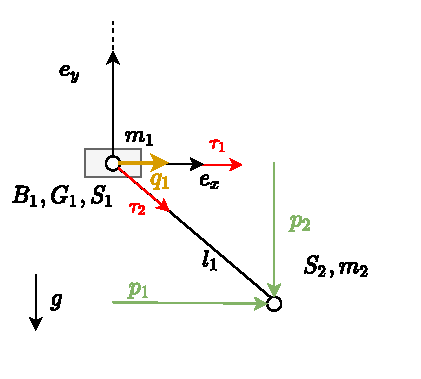
\includegraphics[scale=1]{Pictures/ODE_flatness_analysis_single_crane_diagram}
	\end{center}
	\caption[Kurzbeschreibung für Abbildungsverzeichnis]
	{Langbeschreibung, die gerne auch über mehrer Zeilen gehen darf.}
	\label{fig:single_crane_diagram}
\end{figure}

Die Position der beiden Massenschwerpunkte kann somit wie folgt durch die Koordinaten beschrieben werden:
\begin{equation}
	\mathbf{S}_1 =
	\begin{pmatrix}
		q_1 \\
		0
	\end{pmatrix}, 
	\quad
	\mathbf{S}_2 =
	\begin{pmatrix}
		p_1 \\
		p_2
	\end{pmatrix}.
\end{equation}

Damit ist es möglich die kinetische und potentielle Energie des Systems zu formulieren:
\begin{align}
	T &= \frac{m_1}{2} \dot{\mathbf{S}}_1^T \dot{\mathbf{S}}_1 + \frac{m_2}{2} \dot{\mathbf{S}}_2^T \dot{\mathbf{S}}_2 = \frac{m_{1} \dot{q}_{1}^{2}}{2} + \frac{m_{2} \dot{p}_{1}^{2}}{2} + \frac{m_{2} \dot{p}_{2}^{2}}{2} \\
	V &= m_2 g \ \mathbf{S}_2^T \mathbf{e}_y = m_{2} g p_{2}.
\end{align}

Die Systemgleichungen können durch die Lagrange-Gleichungen zweiter Art zunächst in Abhängigkeit der Komponenten der generalisierten Kraft $Q_i$ bestimmt werden:
\begin{align}
	- Q_{1} + m_{2} \ddot{p}_{1} &= 0\\
	- Q_{2} + g m_{2} + m_{2} \ddot{p}_{2} &= 0\\
	- Q_{3} + m_{1} \ddot{q}_{1} &= 0.
\end{align}

Die Eingangskomponenten $\tau_1$, $\tau_2$ des Systems können können über Stellkräfte vektoriell dargestellt werden:
\begin{equation}
	\mathbf{F}_1 =
	\left(\begin{matrix}
		\tau_{1} \\
		0
	\end{matrix}\right), \quad
	\mathbf{F}_2 =
	\left(\begin{matrix}
		\frac{\tau_{2} \left(p_{1} - q_{1}\right)}{l_{1}}\\
		\frac{p_{2} \tau_{2}}{l_{1}}
	\end{matrix}\right).
\end{equation}

Durch die Anwendung des Prinzips der virtuellen Arbeit ist es möglich, die generalisierte Kraft durch diese Stellkräfte bzw. den Systemeingang auszudrücken:
\begin{equation}
	\mathbf{Q}=
	\left(\begin{matrix}
		\frac{\tau_{2} \left(p_{1} - q_{1}\right)}{l_{1}}\\
		\frac{p_{2} \tau_{2}}{l_{1}}\\
		\tau_{1} - \frac{\tau_{2} \left(p_{1} - q_{1}\right)}{l_{1}}
	\end{matrix}\right).
\end{equation}

Durch einsetzen dieser lässt sich ein abschließender Satz an Systemgleichungen des Einzelkrans bilden:
\begin{align}
	m_{2} \ddot{p}_{1} - \frac{\tau_{2} \left(p_{1} - q_{1}\right)}{l_{1}} &= 0\\
	g m_{2} + m_{2} \ddot{p}_{2} - \frac{p_{2} \tau_{2}}{l_{1}} &= 0\\
	m_{1} \ddot{q}_{1} - \tau_{1} + \frac{\tau_{2} \left(p_{1} - q_{1}\right)}{l_{1}} &= 0.
\end{align}

\section{Analytisches Modell Doppelkran}

\subsection{Ansatz über ein ODE-System}
(Im Folgenden genutztes Notebook: flatness\_notebooks/ODE\_flatness\_analysis.ipynb)

Mittels der Lagrange-Gleichungen zweiter Art wird im Folgenden ein ODE-Modell des Doppelkrans erzeugt. Dabei wird entsprechend der Erläuterungen aus Abschnitt \ref{sec:Lagrange2_theory} vorgegangen. Diese Modellierung hat den Vorteil, dass durch die generalisierte Kraft gerade die Stellkraft im Seil gut abgebildet werden kann sowie keine Zwangsbedingungen im späteren Flachheitsnachweis berücksichtigt werden müssen.

Als aktuierte Koordinate werden zunächst nur die $x$-Verschiebungen $q_1$ und $q_2$ der Laufkatzenpositionen ($\mathbf{B}_1 = \mathbf{G}_1 = \mathbf{S}_1$, $\mathbf{B}_2 = \mathbf{G}_6 = \mathbf{S}_3$) ausgewählt, als passive Koordinaten die absolute Position $(p_1, p_2)$ des Lastschwerpunkts ($\mathbf{S}_2$) sowie die Orientierung der Last $p_3$ gegenüber der Horizontalen. Die variable Seillänge wird mit $l_1$ sowie $l_2$ bezeichnet, die durch die Koordinaten auch mittels:
\begin{align}
	l_1 &= \sqrt{\left(p_{2} - s_{2} \sin{\left(p_{3} \right)}\right)^{2} + \left(p_{1} - q_{1} - s_{2} \cos{\left(p_{3} \right)}\right)^{2}} \\
	l_2 &= \sqrt{\left(p_{2} + s_{2} \sin{\left(p_{3} \right)}\right)^{2} + \left(- l_{0} + p_{1} - q_{2} + s_{2} \cos{\left(p_{3} \right)}\right)^{2}}
\end{align}
ausgedrückt werden kann.

\begin{figure}[ht]
	\begin{center}
		% hier keine Skalierung notwendig, wenn Datei schon mit passender figsize angelegt wurde:
		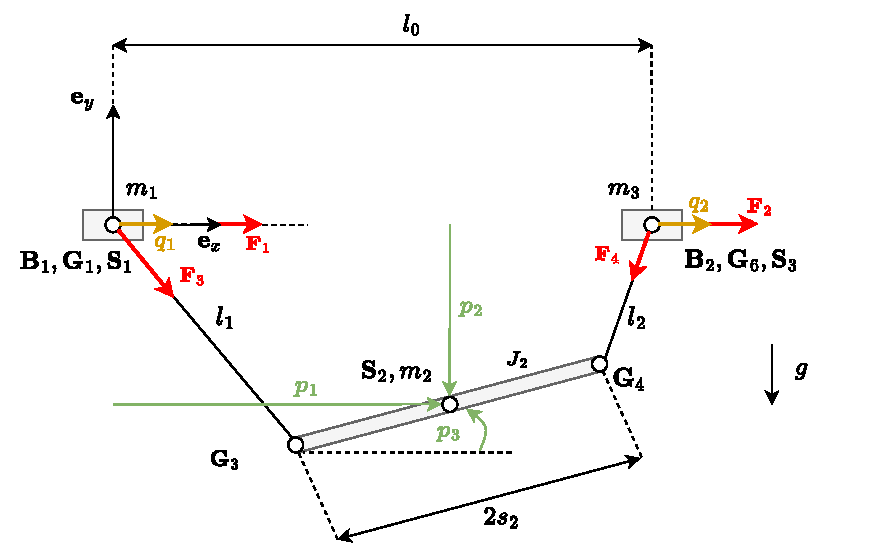
\includegraphics[scale=1]{Pictures/ODE_flatness_analysis_double_crane_diagram}
	\end{center}
	\caption[Kurzbeschreibung für Abbildungsverzeichnis]
	{Langbeschreibung, die gerne auch über mehrer Zeilen gehen darf.}
	\label{fig:double_crane_diagram}
\end{figure}

Die Position der Massenschwerpunkte und Gelenke kann somit wie folgt durch die Koordinaten beschrieben werden:
\begin{equation}
	\mathbf{S}_1 =
	\begin{pmatrix}
		q_1 \\
		0
	\end{pmatrix}, 
	\
	\mathbf{S}_2 =
	\begin{pmatrix}
		p_1 \\
		p_2
	\end{pmatrix},
	\
	\mathbf{S}_3 =
	\begin{pmatrix}
		l_0 + q_2 \\
		0
	\end{pmatrix},
	\
	\mathbf{G}_3 =
	\left(\begin{matrix}
		p_{1} - s_{2} \cos{\left(p_{3} \right)}\\
		p_{2} - s_{2} \sin{\left(p_{3} \right)}
	\end{matrix}\right),
	\
	\mathbf{G}_4 =
	\left(\begin{matrix}
		p_{1} + s_{2} \cos{\left(p_{3} \right)}\\
		p_{2} + s_{2} \sin{\left(p_{3} \right)}
	\end{matrix}\right).
\end{equation}

Damit ist es möglich die kinetische und potentielle Energie des Systems zu formulieren:
\begin{align}
	T &= \frac{m_1}{2} \dot{\mathbf{S}}_1^T \dot{\mathbf{S}}_1 + \frac{m_2}{2} \dot{\mathbf{S}}_2^T \dot{\mathbf{S}}_2 + \frac{J_2}{2} \dot{p}_3^2 + \frac{m_3}{2} \dot{\mathbf{S}}_3^T \dot{\mathbf{S}}_3 \nonumber \\  
	&= \frac{J_{2} \dot{p}_{3}^{2}}{2} + \frac{m_{1} \dot{q}_{1}^{2}}{2} + \frac{m_{2} \dot{p}_{1}^{2}}{2} + \frac{m_{2} \dot{p}_{2}^{2}}{2} + \frac{m_{3} \dot{q}_{2}^{2}}{2} \\
	V &= m_2 g \ \mathbf{S}_2^T \mathbf{e}_y = m_{2} g p_{2}.
\end{align}

Die Systemgleichungen können durch die Lagrange-Gleichungen zweiter Art zunächst in Abhängigkeit der Komponenten der generalisierten Kraft $Q_i$ bestimmt werden:
\begin{align}
	- Q_{1} + m_{2} \ddot{p}_{1} &= 0\\
	- Q_{2} + g m_{2} + m_{2} \ddot{p}_{2} &= 0\\
	J_{2} \ddot{p}_{3} - Q_{3} &= 0\\
	- Q_{4} + m_{1} \ddot{q}_{1} &= 0\\
	- Q_{5} + m_{3} \ddot{q}_{2} &= 0.
\end{align}

Die Komponenten des Systemeingangs $\mathbf{\tau}$ können über Stellkräfte vektoriell dargestellt werden:
\begin{equation}
	\mathbf{F}_1 =
	\left(\begin{matrix}
		\tau_{1} \\
		0
	\end{matrix}\right), \
	\mathbf{F}_2 =
	\left(\begin{matrix}
		\tau_{2} \\
		0
	\end{matrix}\right), \
	\mathbf{F}_3 =
	\left(\begin{matrix}
		\frac{\tau_{3} \left(p_{1} - q_{1} - s_{2} \cos{\left(p_{3} \right)}\right)}{l_{1}}\\
		\frac{\tau_{3} \left(p_{2} - s_{2} \sin{\left(p_{3} \right)}\right)}{l_{1}}
	\end{matrix}\right), \
	\mathbf{F}_4 =
	\left(\begin{matrix}
		\frac{\tau_{4} \left(- l_{0} + p_{1} - q_{2} + s_{2} \cos{\left(p_{3} \right)}\right)}{l_{2}}\\
		\frac{\tau_{4} \left(p_{2} + s_{2} \sin{\left(p_{3} \right)}\right)}{l_{2}}
	\end{matrix}\right).
\end{equation}

Durch die Anwendung des Prinzips der virtuellen Arbeit ist es möglich, die generalisierte Kraft durch diese Stellkräfte bzw. den Systemeingang auszudrücken:
\begin{equation}
	\mathbf{Q}=
	\left(\begin{smallmatrix}
		\frac{\tau_{4} \left(- l_{0} + p_{1} - q_{2} + s_{2} \cos{\left(p_{3} \right)}\right)}{l_{2}} + \frac{\tau_{3} \left(p_{1} - q_{1} - s_{2} \cos{\left(p_{3} \right)}\right)}{l_{1}}\\
		\frac{\tau_{4} \left(p_{2} + s_{2} \sin{\left(p_{3} \right)}\right)}{l_{2}} + \frac{\tau_{3} \left(p_{2} - s_{2} \sin{\left(p_{3} \right)}\right)}{l_{1}}\\
		\frac{s_{2} \tau_{4} \left(p_{2} + s_{2} \sin{\left(p_{3} \right)}\right) \cos{\left(p_{3} \right)}}{l_{2}} - \frac{s_{2} \tau_{4} \left(- l_{0} + p_{1} - q_{2} + s_{2} \cos{\left(p_{3} \right)}\right) \sin{\left(p_{3} \right)}}{l_{2}} - \frac{s_{2} \tau_{3} \left(p_{2} - s_{2} \sin{\left(p_{3} \right)}\right) \cos{\left(p_{3} \right)}}{l_{1}} + \frac{s_{2} \tau_{3} \left(p_{1} - q_{1} - s_{2} \cos{\left(p_{3} \right)}\right) \sin{\left(p_{3} \right)}}{l_{1}}\\
		\tau_{1} - \frac{\tau_{3} \left(p_{1} - q_{1} - s_{2} \cos{\left(p_{3} \right)}\right)}{l_{1}}\\
		\tau_{2} - \frac{\tau_{4} \left(- l_{0} + p_{1} - q_{2} + s_{2} \cos{\left(p_{3} \right)}\right)}{l_{2}}
	\end{smallmatrix}\right).
\end{equation}

Durch einsetzen dieser lässt sich ein abschließender Satz an Systemgleichungen des Einzelkrans bilden:
\begin{flalign}
	&m_{2} \ddot{p}_{1} - \frac{\tau_{4} \left(- l_{0} + p_{1} - q_{2} + s_{2} \cos{\left(p_{3} \right)}\right)}{l_{2}} - \frac{\tau_{3} \left(p_{1} - q_{1} - s_{2} \cos{\left(p_{3} \right)}\right)}{l_{1}} = 0\\
	&g m_{2} + m_{2} \ddot{p}_{2} - \frac{\tau_{4} \left(p_{2} + s_{2} \sin{\left(p_{3} \right)}\right)}{l_{2}} - \frac{\tau_{3} \left(p_{2} s_{2} \sin{\left(p_{3} \right)}\right)}{l_{1}} = 0\\
	&J_{2} \ddot{p}_{3} - \frac{s_{2} \tau_{4} \left(p_{2} + s_{2} \sin{\left(p_{3} \right)}\right) \cos{\left(p_{3} \right)}}{l_{2}} + \frac{s_{2} \tau_{4} \left(- l_{0} + p_{1} - q_{2} + s_{2} \cos{\left(p_{3} \right)}\right) \sin{\left(p_{3} \right)}}{l_{2}} \nonumber\\ 
	&+ \frac{s_{2} \tau_{3} \left(p_{2} - s_{2} \sin{\left(p_{3} \right)}\right) \cos{\left(p_{3} \right)}}{l_{1}} - \frac{s_{2} \tau_{3} \left(p_{1} - q_{1} - s_{2} \cos{\left(p_{3} \right)}\right) \sin{\left(p_{3} \right)}}{l_{1}} = 0\\
	&m_{1} \ddot{q}_{1} - \tau_{1} + \frac{\tau_{3} \left(p_{1} - q_{1} - s_{2} \cos{\left(p_{3} \right)}\right)}{l_{1}} = 0\\
	&m_{3} \ddot{q}_{2} - \tau_{2} + \frac{\tau_{4} \left(- l_{0} + p_{1} - q_{2} + s_{2} \cos{\left(p_{3} \right)}\right)}{l_{2}} = 0.
\end{flalign}

Alternativ kann das Doppelkransystem auch eingangsaffin im Zustandsraum beschrieben werden:
\begin{align}
	\dot{\mathbf{x}} &= \mathbf{f}(\mathbf{x}) + \mathbf{g}(\mathbf{x}) \mathbf{\tau}, \nonumber \\ \mathbf{x} &= (p_{1},	p_{2}, p_{3}, q_{1}, q_{2}, \dot{p}_{1}, \dot{p}_{2}, \dot{p}_{3}, \dot{q}_{1}, \dot{q}_{2})^T, \nonumber \\
	\mathbf{f}(\mathbf{x}) &= 
	(\dot{p}_{1}, \dot{p}_{2}, \dot{p}_{3}, \dot{q}_{1}, \dot{q}_{2}, 0, -g, 0, 0, 0)^T, \nonumber \\ 
	\mathbf{g}(\mathbf{x}) &=
	\left(\begin{matrix}
		0 & 0 & 0 & 0\\
		0 & 0 & 0 & 0\\
		0 & 0 & 0 & 0\\
		0 & 0 & 0 & 0\\
		0 & 0 & 0 & 0\\
		0 & 0 & \frac{p_{1} - q_{1} - s_{2} \cos{\left(p_{3} \right)}}{l_{1} m_{2}} & \frac{- l_{0} + p_{1} - q_{2} + s_{2} \cos{\left(p_{3} \right)}}{l_{2} m_{2}}\\
		0 & 0 & \frac{p_{2} - s_{2} \sin{\left(p_{3} \right)}}{l_{1} m_{2}} & \frac{p_{2} + s_{2} \sin{\left(p_{3} \right)}}{l_{2} m_{2}}\\
		0 & 0 & \frac{s_{2} \left(p_{1} \sin{\left(p_{3} \right)} - p_{2} \cos{\left(p_{3} \right)} - q_{1} \sin{\left(p_{3} \right)}\right)}{J_{2} l_{1}} & \frac{s_{2} \left(l_{0} \sin{\left(p_{3} \right)} - p_{1} \sin{\left(p_{3} \right)} + p_{2} \cos{\left(p_{3} \right)} + q_{2} \sin{\left(p_{3} \right)}\right)}{J_{2} l_{2}}\\
		\frac{1}{m_{1}} & 0 & \frac{- p_{1} + q_{1} + s_{2} \cos{\left(p_{3} \right)}}{l_{1} m_{1}} & 0\\
		0 & \frac{1}{m_{3}} & 0 & \frac{l_{0} - p_{1} + q_{2} - s_{2} \cos{\left(p_{3} \right)}}{l_{2} m_{3}}
	\end{matrix}\right).
\end{align}

\subsection{Ansatz über ein DAE-System}
(Im Folgenden genutztes Notebook: double\_crane\_notebooks/DAE\_double\_crane\_cartesian.ipynb)

Mittels der Lagrange-Gleichungen erster Art wird im Folgenden ein DAE-Modell des Doppelkrans erzeugt. Dabei wird entsprechend der Erläuterungen aus Abschnitt \ref{sec:Lagrange1_theory} vorgegangen. Diese Modellierung hat den Vorteil, dass durch die Einprägung von Zwangsbedingungen die kinematische Schleife wegen der gemeinsamen Last intuitiv abgebildet werden kann. Aufgrund der algebraischen Gleichungen würde sich ein Flachheitsnachweis anders als bei den ODE-Systemen gestalten. Es wird einzig eine horizontale Aktuierung der Laufkatzen durch den Eingang $\mathbf{\tau} = (\tau_{1}, \tau_{2})^T$ betrachtet. Für eine spätere effiziente Simulation mit aktuierten Seilwinden wäre gerade bei konstanten Längen dieser eine Umformulierung des Problems mit den Längen als Stellgröße sinnvoll. (Quelle: Buch von Rudolf S.21 -> Nextcloud Flachheit/fotos ???)

Als aktuierte Koordinate werden nur die $x$-Verschiebungen $q_1$ und $q_2$ der Laufkatzenpositionen ($\mathbf{B}_1 = \mathbf{G}_1 = \mathbf{S}_1$, $\mathbf{B}_2 = \mathbf{G}_4 = \mathbf{S}_5$) ausgewählt, als passive Koordinaten die absolute Position $(p_1, p_2)$ des Gelenks $\mathbf{G}_2 (= \mathbf{S}_2)$ sowie $(p_3, p_4)$ des Gelenks $\mathbf{G}_3 = (\mathbf{S}_4)$. 

Für konstante Seillängen können folgende Zwangsbedingungen formuliert werden:
\begin{align}
	l_{1} - \sqrt{p_{2}^{2} + \left(p_{1} - q_{1}\right)^{2}} &= 0\\
	l_{2} - \sqrt{p_{4}^{2} + \left(- l_{0} + p_{3} - q_{2}\right)^{2}} &= 0.	
\end{align}

Die konstante Lastlänge wird durch
\begin{equation}
	2 s_{3} - \sqrt{\left(p_{1} - p_{3}\right)^{2} + \left(p_{2} - p_{4}\right)^{2}}
\end{equation}
ausgedrückt.

\begin{figure}[ht]
	\begin{center}
		% hier keine Skalierung notwendig, wenn Datei schon mit passender figsize angelegt wurde:
		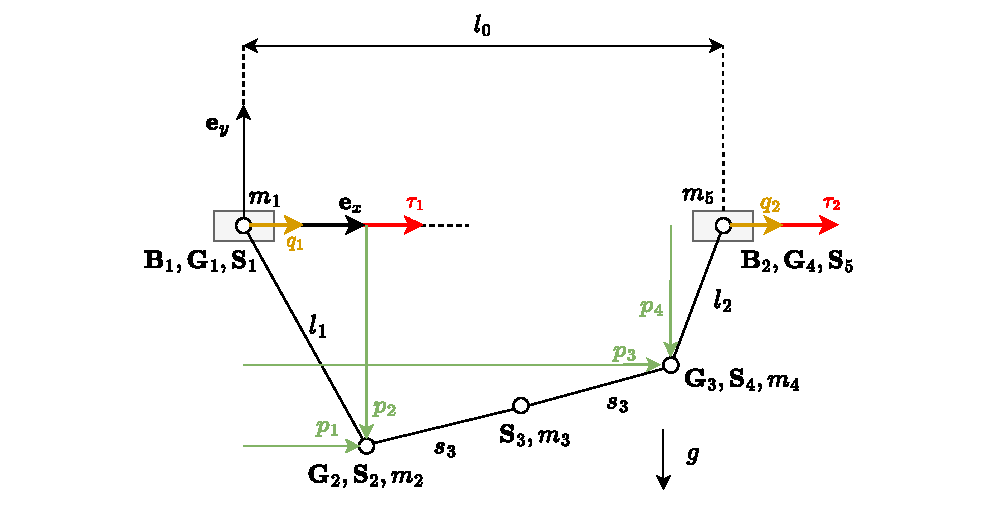
\includegraphics[scale=1]{Pictures/DAE_double_crane_cartesian_diagram.pdf}
	\end{center}
	\caption[Kurzbeschreibung für Abbildungsverzeichnis]
	{Langbeschreibung, die gerne auch über mehrer Zeilen gehen darf.}
	\label{fig:DAE_double_crane_diagram}
\end{figure}

Die Position der Massenschwerpunkte und Gelenke kann somit wie folgt durch die Koordinaten beschrieben werden:
\begin{align}
	\mathbf{S}_1 =
	\begin{pmatrix}
		q_1 \\
		0
	\end{pmatrix}, 
	\
	\mathbf{S}_2 =
	\begin{pmatrix}
		p_1 \\
		p_2
	\end{pmatrix},
	\
	\mathbf{S}_3 =
	\frac{1}{2}(\mathbf{S}_2 + \mathbf{S}_4) =
	\frac{1}{2}
	\begin{pmatrix}
		p_1 + p_3 \\
		p_2 + p_4
	\end{pmatrix},
	\nonumber \\
	\mathbf{S}_4 =
	\left(\begin{matrix}
		p_3 \\
		p_4
	\end{matrix}\right),
	\
	\mathbf{S}_5 =
	\left(\begin{matrix}
		l_0 + q_2 \\
		0
	\end{matrix}\right).
\end{align}

Es ist notwendig, dass alle abgeleiteten Koordinaten in der kinetischen Energie $T$ (Theoretische Begründung wieso !?!) vorhanden sind. Dies wäre bei einer Modellierung der Last mit homogener Masseverteilung und Trägheitsmoment nicht der Fall. Deshalb wird die Last durch ein System aus drei Massen ($m_2$, $m_3$, $m_4$) beschrieben, das sich simulativ äquivalent verhalten sollte und folgenden Gleichungen genügt:
\begin{align}
	m_{\mathrm{ges}} &= m_2 + m_3 + m_4\\
	m_2 &= m_4\\
	J &= m_2 s_3^2 + m_4 s_3^2 = 2 m_2 s_3^2\\
	\Rightarrow m_2 &= m_4 = \frac{J}{2 s_3^2} \\
	\Rightarrow m_3 &= m_{\mathrm{ges}} - m_2 -m_4.
\end{align}

Die größen $m_{\mathrm{ges}}$ und $J$ beziehen sich auf die identifizierten Systemparameter, die so auch bei der Modellbildung des Doppelkrans als ODE-System genutzt wurden.

Somit ist es möglich die kinetische und potentielle Energie des Systems zu formulieren:
\begin{align}
	T &= \frac{m_1}{2} \dot{\mathbf{S}}_1^T \dot{\mathbf{S}}_1 + \frac{m_2}{2} \dot{\mathbf{S}}_2^T \dot{\mathbf{S}}_2 + \frac{m_3}{2} \dot{\mathbf{S}}_3^T \dot{\mathbf{S}}_3 + \frac{m_4}{2} \dot{\mathbf{S}}_4^T \dot{\mathbf{S}}_4 + \frac{m_5}{2} \dot{\mathbf{S}}_5^T \dot{\mathbf{S}}_5 \nonumber \\  
	&= \frac{m_{1} \dot{q}_{1}^{2}}{2} + \frac{m_{2} \dot{p}_{1}^{2}}{2} + \frac{m_{2} \dot{p}_{2}^{2}}{2} + \frac{m_{3} \cdot 0.25 \left(\dot{p}_{1} + \dot{p}_{3}\right)^{2}}{2} + \frac{m_{3} \cdot 0.25 \left(\dot{p}_{2} + \dot{p}_{4}\right)^{2}}{2} \nonumber \\
	&+ \frac{m_{4} \dot{p}_{3}^{2}}{2} + \frac{m_{4} \dot{p}_{4}^{2}}{2} + \frac{m_{5} \dot{q}_{2}^{2}}{2} \\
	V &= (m_2 \ g \ \mathbf{S}_2^T + m_3 \ g \ \mathbf{S}_3^T + m_4 \ g \ \mathbf{S}_4^T) \mathbf{e}_y \nonumber \\ &= g \left(m_{2} p_{2} + m_{3} \left(0.5 p_{2} + 0.5 p_{4}\right) + m_{4} p_{4}\right).
\end{align}

Unter Nutzung der Lagrange-Multiplikatoren $\lambda_j$ lassen sich die Systemgleichungen ausdrücken:
\begin{flalign}
	&- \frac{\lambda_{1} p_{1}}{\sqrt{p_{2}^{2} + \left(p_{1} - q_{1}\right)^{2}}} + \frac{\lambda_{1} q_{1}}{\sqrt{p_{2}^{2} + \left(p_{1} - q_{1}\right)^{2}}} - \frac{\lambda_{2} p_{1}}{\sqrt{\left(p_{1} - p_{3}\right)^{2} + \left(p_{2} - p_{4}\right)^{2}}} \nonumber \\
	&+ \frac{\lambda_{2} p_{3}}{\sqrt{\left(p_{1} - p_{3}\right)^{2} + \left(p_{2} - p_{4}\right)^{2}}} + m_{2} \ddot{p}_{1} + 0.25 m_{3} \ddot{p}_{1} + 0.25 m_{3} \ddot{p}_{3} = 0\\
	&g m_{2} + 0.5 g m_{3} - \frac{\lambda_{1} p_{2}}{\sqrt{p_{2}^{2} + \left(p_{1} - q_{1}\right)^{2}}} - \frac{\lambda_{2} p_{2} + \lambda_{2} p_{4}}{\sqrt{\left(p_{1} - p_{3}\right)^{2} + \left(p_{2} - p_{4}\right)^{2}}} \nonumber \\
	&+ m_{2} \ddot{p}_{2} + 0.25 m_{3} \ddot{p}_{2} + 0.25 m_{3} \ddot{p}_{4} = 0\\
	&\frac{\lambda_{2} \left(p_{1} - p_{3}\right)}{\sqrt{\left(p_{1} - p_{3}\right)^{2} + \left(p_{2} - p_{4}\right)^{2}}} + \frac{\lambda_{3} \left(l_{0} - p_{3} + q_{2}\right)}{\sqrt{p_{4}^{2} + \left(l_{0} - p_{3} + q_{2}\right)^{2}}} \noindent \\
	&+ \frac{m_{3} \left(0.5 \ddot{p}_{1} + 0.5 \ddot{p}_{3}\right)}{2} + m_{4} \ddot{p}_{3} = 0\\
	&0.5 g m_{3} + g m_{4} + \frac{\lambda_{2} p_{2}}{\sqrt{\left(p_{1} - p_{3}\right)^{2} + \left(p_{2} - p_{4}\right)^{2}}} - \frac{\lambda_{2} p_{4}}{\sqrt{\left(p_{1} - p_{3}\right)^{2} + \left(p_{2} - p_{4}\right)^{2}}} \nonumber \\ 
	&- \frac{\lambda_{3} p_{4}}{\sqrt{p_{4}^{2} + \left(l_{0} - p_{3} + q_{2}\right)^{2}}} + 0.25 m_{3} \ddot{p}_{2} + 0.25 m_{3} \ddot{p}_{4} + m_{4} \ddot{p}_{4} = 0\\
	&\frac{\lambda_{1} \left(p_{1} - q_{1}\right) + \sqrt{p_{2}^{2} + \left(p_{1} - q_{1}\right)^{2}} \left(m_{1} \ddot{q}_{1} - \tau_{1}\right)}{\sqrt{p_{2}^{2} + \left(p_{1} - q_{1}\right)^{2}}} = 0\\
	&\frac{- \lambda_{3} \left(l_{0} - p_{3} + q_{2}\right) + \sqrt{p_{4}^{2} + \left(l_{0} - p_{3} + q_{2}\right)^{2}} \left(m_{5} \ddot{q}_{2} - \tau_{2}\right)}{\sqrt{p_{4}^{2} + \left(l_{0} - p_{3} + q_{2}\right)^{2}}} = 0.
\end{flalign}

\section{Systemidentifikation}

Die meisten in den Modellen vorkommenden Systemparameter sind geometrischer Natur oder Massen und lassen sich durch Messen mit einem Lineal oder einer Wage bestimmen. Nur das Trägheitsmoment der Last kann entsprechend der Annahme eines Quaders mit homogener Masseverteilung und Rotationsachse durch seinen Mittelpunkt, die in die Ebene zeigt, berechnet werden \cite{LastTraegheit}:
\begin{equation}
	J = \frac{1}{12} m_2 ((2 s_2)^2 + h^2).
\end{equation}

Dabei entspricht $h$ der Höhe der Last, welche zu $h = 90$ mm
bestimmt wurde.

\begin{table}[htbp]%
	\centering
	\caption{Physikalische Parameter des Doppelkrandemonstratorsystems.}
	\label{tab:relative_degrees}
	\begin{tabular}{c c c} 
		Parameter & Bezeichnung im ODE-Modell & Wert \\ 
		\hline
		Masse Laufkatze 1 & $m_1$ & 0,45 \si{\kg} \\
		Masse Laufkatze 2 & $m_3$ & 0,45 \si{\kg} \\
 		Masse Last & $m_2$ & 0,557 \si{\kg} \\
		Länge Last & $2 s_2$ & 0,15 \si{\m} \\
		Initialer Laufkatzenabstand & $l_0$ & 0,3 \si{\m} \\
		Trägheitsmoment Last & $J_2$ & 0,00455 $\si{\kg\m^2}$ \\
		\bottomrule
	\end{tabular}
\end{table}

\chapter{Flachheitsanalyse}

\section{Definition differenzieller Flachheit}\label{sec:Def_flatness}

Ein System der Form $\dot{\mathbf{x}} = \mathbf{F}(\mathbf{x}, \mathbf{u})$ mit $\mathbf{F}, \mathbf{x} \in \mathbb{R}^n$ und $\mathbf{u} \in \mathbb{R}^m$ ist (differenziell) flach, falls ein $m$-Tupel $y := (y_1, ..., y_m)^T$ sowie glatte Funktionen $\mathbf{\Psi}$, $\mathbf{\Theta}$ existieren, so dass:
\begin{align}
\mathbf{x} &= \mathbf{\Psi}(\mathbf{y}, \dot{\mathbf{y}}, ..., \mathbf{y}^{(n_x)}) \text{ mit } n_x < \infty \text{ und } \\
\mathbf{u} &= \mathbf{\Theta}(\mathbf{y}, \dot{\mathbf{y}}, ..., \mathbf{y}^{(n_u)}) \text{ mit } n_u < \infty.
\end{align}

Dabei ist $\mathbf{y}$ ein flacher Ausgang \cite[S. 185]{NLRT_Roebenack}. 

Aus der Existenz eines flachen Ausgangs folgt, dass die Systemgrößen bestehend aus dem Zustand $\mathbf{x}$ und Eingang $\mathbf{u}$ eindeutig aus dem flachen Ausgang $\mathbf{y}$ und einer endlichen Anzahl dessen Zeitableitungen berechnet werden können, also keine Integrale dafür gelöst werden müssen. Eine alternative Formulierung des Flachheitsbegriffs verzichtet auf die Angabe der gleichen Dimension $m$ von Eingang und flachem Ausgang, fordert aber die differenzielle Unabhängigkeit der Komponenten von $\mathbf{y}$.

Die Existenzbedingungen eines flachen Ausgangs sind bei Eingrößensystemen bekannt, allerdings ist der systematische Flachheitsnachweis und die Berechnung eines
flachen Ausgangs bei Mehrgrößensystemen im Allgemeinen nicht abschließend gelöst.

\section{Flachheitsanalyse von MIMO-Systemen}

Im Folgenden wird ein prinzipielles praktisches Vorgehen zur Bestimmung flacher Ausgänge von Mehrgrößensystemen sowie zur Parametrisierung der Systemgrößen anhand solcher flachen Ausgänge skizziert werden. Für eine mathematisch fundierte und systematische Herangehensweise sei auf den Beitrag \cite{Fritzsche2016} verwiesen.

Es sei ein nichtlineares Mehrgrößensystem der Form aus Abschnitt \ref{sec:Def_flatness} gegeben. Dessen Eingang $\mathbf{u}$ kommt in affiner Form vor und könne mittels der Systemgleichungen eliminiert werden, so dass ein autonomes System aus $p = n - m$ Gleichungen folgt. Diese Gleichungen werden wiederum zur Elimination $p$ übriger Zustandskomponenten genutzt, so dass sich ein flacher Ausgang $\mathbf{y}$ der Dimension $n - p = m$ ergibt. 

Zur Auswahl einer geeigneten Systemgleichung und Eingangskomponente für die Elimination bietet sich die Bildung der Jacobi-Matrix $\mathbf{J}_i$ der zu diesem Zeitpunkt noch $i$ betrachteten Systemgleichungen bezüglich des Eingangs $\mathbf{u}_{m-(n-i)}$ an. Dabei sind die zu den Matrixzeilen korrespondierenden Gleichungen geeignet, in denen nur ein isolierter Spalteneintrag $\varepsilon \neq 0$ steht, also weitere Einträge der Spalte Null sind:
\begin{equation}
	\begin{pmatrix}
	* & \cdots & * & 0 & * & \cdots & *\\
	\vdots & \ddots & \vdots & \vdots & \vdots & \ddots & \vdots \\
	* & \cdots & * & 0 & * & \cdots & *  \\
	* & \cdots & * & \varepsilon & * & \cdots & * \\
	* & \cdots & * & 0 & * & \cdots & *  \\
	\vdots & \ddots & \vdots & \vdots & \vdots & \ddots & \vdots \\
	* & \cdots & * & 0 & * & \cdots & *\\
	\end{pmatrix}.
\end{equation}

Falls keine solcher Spalten zu finden ist, kann eine Transformation $\mathbf{T}$ der Systemgleichungen durchgeführt werden, welche mittels linkem Orthokomplement $\mathbf{J}_i^{L \perp}$ und linker Pseudoinverser $\mathbf{J}_i^{L +}$ der Jacobi-Matrix das System in eine geeignete Form überführt \cite[Abschnitt 2.1.2]{Fritzsche2016}:
\begin{equation}
	\mathbf{T} \mathbf{J}_i = 
	\begin{pmatrix}
		\mathbf{I}_{m-(n-i)} \\
		\mathbf{0}_{(n-m) \times (m-(n-i))}
	\end{pmatrix}.
\end{equation}

Wobei $\mathbf{T}$ über die Eigenschaften von $\mathbf{J}_i^{L +}$ und  $\mathbf{J}_i^{L \perp}$ folgendermaßen gebildet werden kann:
\begin{align}
	\mathbf{J}_i^{L +} \mathbf{J}_i = \mathbf{I}_i \\
	\mathbf{J}_i^{L \perp} \mathbf{J}_i = \mathbf{0}_{(n-m) \times (m-(n-i))} \\
	\Rightarrow \mathbf{T} = 
	\begin{pmatrix}
		\mathbf{J}_i^{L +} \\
		\mathbf{J}_i^{L \perp}
	\end{pmatrix} .
\end{align}

Nachdem die Eingangskomponenten aus den Systemgleichungen eliminiert wurden kann analog durch Bildung einer Jacobi-Matrix bezüglich der noch vorhandenen Systemgrößen vorgenommen werden. Der Flache Ausgang $\mathbf{y}$ besteht aus der Menge an Systemgrößen, welche nach Elimination aller Gleichungen übrig ist. Mittels der Zusammenhänge aus den Systemgleichungen können nach \ref{sec:Def_flatness} alle Systemgrößen allein durch $(\mathbf{y}, \dot{\mathbf{y}}, \ddot{\mathbf{y}}, ...)$ parametrisiert werden.

\section{Anwendung Flachheitsanalyse am Einzelkran}
Herangezogen: ODE Modell des Einzelkrans aus Lagrange 2 \\ (flatness\_notebooks/ODE\_flatness\_analysis\_single\_crane.ipynb) \\
-> Aus analytischer Modellbildung des Einzelkransystems folgen die 3 Systemgleichungen:
\begin{align}
	m_{2} \ddot{p}_{1} - \frac{\tau_{2} \left(p_{1} - q_{1}\right)}{\sqrt{p_{2}^{2} + \left(p_{1} - q_{1}\right)^{2}}} = 0\label{single_flat_syseq1}\\
	g m_{2} + m_{2} \ddot{p}_{2} - \frac{p_{2} \tau_{2}}{\sqrt{p_{2}^{2} + \left(p_{1} - q_{1}\right)^{2}}} = 0\label{single_flat_syseq2}\\
	m_{1} \ddot{q}_{1} - \tau_{1} + \frac{\tau_{2} \left(p_{1} - q_{1}\right)}{\sqrt{p_{2}^{2} + \left(p_{1} - q_{1}\right)^{2}}} = 0\label{single_flat_syseq3}
\end{align}
- Bildung der Jacobi-Matrix dieser Gleichungen bezüglich $\mathbf{\tau}$:
\begin{equation}
	\mathbf{J}_3 =
	\left(\begin{matrix}
		0 & - \frac{p_{1} - q_{1}}{\sqrt{p_{2}^{2} + \left(p_{1} - q_{1}\right)^{2}}}\\
		0 & - \frac{p_{2}}{\sqrt{p_{2}^{2} + \left(p_{1} - q_{1}\right)^{2}}}\\
		-1 & \frac{p_{1} - q_{1}}{\sqrt{p_{2}^{2} + \left(p_{1} - q_{1}\right)^{2}}}
	\end{matrix}\right)
\end{equation}
- dabei ist zu erkennen, dass in der ersten Spalte der Jacobi-Matrix die Eingangskomponente $\tau_{1}$ isoliert vorkommt, also durch die korrespondierende dritte Systemgleichung \ref{single_flat_syseq3} bestimmt werden kann. \\
-> Dementsprechend kann die letzte Zeile von $\mathbf{J}_3$ eliminiert werden. \\
- Die verbleibenden ersten beiden Systemgleichungen \ref{single_flat_syseq1} und \ref{single_flat_syseq2} enthalten jeweils die Eingangskomponente $\tau_2$. Da in der zweiten Gleichung \ref{single_flat_syseq2} $\tau_2$ allein durch $p_2$ und die Ableitung $\ddot{p}_2$ dargestellt werden kann, wird diese Gleichung zur Elimination dieser Eingangskomponente genutzt, eine vorweggenommene Parametrisierung durch $p_2$ und $\ddot{p}_2$ ergibt:
\begin{equation}
	\label{eq:pre_single_crane_tau2_w_q1}
	\tau_2 = \frac{l_{1} m_{2} \left(g + \ddot{p}_{2}\right)}{p_{2}}.
\end{equation}

- Dabei ist zu bemerken, dass in dieser Beschreibung von $\tau2$ die Koordinaten $p_1, p_2, q_1$ zusätzlich durch $l_1$ enthalten sind. Diese können nach Parametrisierung durch einen flachen Ausgang anschließend ersetzt werden. 

- Die letzte verbleibende Systemgleichung \ref{single_flat_syseq1} weist nach Substitution des soeben ermittelten $\tau_2$ nur noch die Systemgrößen bzw. Ableitungen $p1, \ddot{p}_1, p2, \ddot{p}_2, q_1$ auf. Damit bietet sich die Elimination des allein algebraisch vorkommenden $q_1$ und auch an dieser stelle Vorwegnahme der Parametrisierung durch $p_1, p_2$ und deren Ableitungen an: 
\begin{equation}
	q_1 = \frac{p_{1} \left(g + \ddot{p}_{2}\right) - p_{2} \ddot{p}_{1}}{g + \ddot{p}_{2}}.
\end{equation}

Somit kann die Substitution von $q_1$ in der flachen Darstellung \ref{eq:pre_single_crane_tau2_w_q1} von $\tau_2$ erfolgen:
\begin{equation}
	\tau_2 =
	\frac{m_{2} \sqrt{\frac{p_{2}^{2} \left(g + \ddot{p}_{2}\right)^{2} + \left(- g p_{1} - p_{1} \ddot{p}_{2} + p_{1} \left(g + \ddot{p}_{2}\right) + p_{2} \ddot{p}_{1}\right)^{2}}{\left(g + \ddot{p}_{2}\right)^{2}}} \left(g + \ddot{p}_{2}\right)}{p_{2}}.
\end{equation}

Um abschließend die zuerst eliminierte Eingangskomponente $\tau_1$ ebenso auszudrücken, wird nach Gleichung \ref{single_flat_syseq3} die zweite zeitliche Ableitung $\ddot{q}_1$ benötigt:
\begin{align}
	\begin{split}
	\ddot{q}_1 &=
	\frac{-2 \dddot{p}_{2} \left(g + \ddot{p}_{2}\right) \left(p_{1} \dddot{p}_{2} - p_{2} \dddot{p}_{1} - \ddot{p}_{1} \dot{p}_{2} + \dot{p}_{1} \left(g + \ddot{p}_{2}\right)\right) }{\left(g + \ddot{p}_{2}\right)^{3}} \\	
	&+ \frac{\left(g + \ddot{p}_{2}\right)^{2} \left(p_{1} \ddddot{p}_{2} - p_{2} \ddddot{p}_{1} - 2 \dddot{p}_{1} \dot{p}_{2} + 2 \dddot{p}_{2} \dot{p}_{1} - \ddot{p}_{1} \ddot{p}_{2} + \ddot{p}_{1} \left(g + \ddot{p}_{2}\right)\right)}{\left(g + \ddot{p}_{2}\right)^{3}}\\	
	&- \frac{\left(p_{1} \left(g + \ddot{p}_{2}\right) - p_{2} \ddot{p}_{1}\right) \left(\ddddot{p}_{2} \left(g + \ddot{p}_{2}\right) - 2 \dddot{p}_{2}^{2}\right)}{\left(g + \ddot{p}_{2}\right)^{3}}.
	\end{split}
\end{align}

Somit folgt:
\begin{align}
	\begin{split}
	\tau_1 &=
	\frac{- m_{1} 2 \dddot{p}_{2} \left(g + \ddot{p}_{2}\right) \left(p_{1} \dddot{p}_{2} - p_{2} \dddot{p}_{1} - \ddot{p}_{1} \dot{p}_{2} + \dot{p}_{1} \left(g + \ddot{p}_{2}\right)\right)}{\left(g + \ddot{p}_{2}\right)^{3}} \\	
	&+ \frac{- m_{1} \left(g + \ddot{p}_{2}\right)^{2} \left(- p_{1} \ddddot{p}_{2} + p_{2} \ddddot{p}_{1} + 2 \dddot{p}_{1} \dot{p}_{2} - 2 \dddot{p}_{2} \dot{p}_{1} + \ddot{p}_{1} \ddot{p}_{2} - \ddot{p}_{1} \left(g + \ddot{p}_{2}\right)\right)}{\left(g + \ddot{p}_{2}\right)^{3}} \\
	&+ \frac{-m_1 \left(p_{1} \left(g + \ddot{p}_{2}\right) - p_{2} \ddot{p}_{1}\right) \left(\ddddot{p}_{2} \left(g + \ddot{p}_{2}\right) - 2 \dddot{p}_{2}^{2}\right)}{\left(g + \ddot{p}_{2}\right)^{3}} + \frac{m_{2} \ddot{p}_{1} \left(g + \ddot{p}_{2}\right)^{3}}{\left(g + \ddot{p}_{2}\right)^{3}}
	\end{split}
\end{align}

Somit ist durch diese Parametrisierung gezeigt, dass es sich bei $\mathbf{y} = (p_1, p_2)^T$ um einen flachen Ausgang handelt.

\section{Anwendung Flachheitsanalyse am Doppelkran}

Herangezogen: ODE Modell des Gantrys aus Lagrange 2 \\ (flatness\_notebooks/ODE\_flatness\_analysis\_control.ipynb) \\
-> Aus analytischer Modellbildung des Doppelkransystems folgen die 5 Systemgleichungen:
\begin{flalign}
	&m_{2} \ddot{p}_{1} - \frac{\tau_{4} \left(- l_{0} + p_{1} - q_{2} + s_{2} \cos{\left(p_{3} \right)}\right)}{l_{2}} - \frac{\tau_{3} \left(p_{1} - q_{1} - s_{2} \cos{\left(p_{3} \right)}\right)}{l_{1}} = 0 \label{double_flat_syseq1}\\
	&g m_{2} + m_{2} \ddot{p}_{2} - \frac{\tau_{4} \left(p_{2} + s_{2} \sin{\left(p_{3} \right)}\right)}{l_{2}} - \frac{\tau_{3} \left(p_{2} - s_{2} \sin{\left(p_{3} \right)}\right)}{l_{1}} = 0 \label{double_flat_syseq2}\\
	&J_{2} \ddot{p}_{3} - \frac{s_{2} \tau_{4} \left(p_{2} + s_{2} \sin{\left(p_{3} \right)}\right) \cos{\left(p_{3} \right)}}{l_{2}} + \frac{s_{2} \tau_{4} \left(- l_{0} + p_{1} - q_{2} + s_{2} \cos{\left(p_{3} \right)}\right) \sin{\left(p_{3} \right)}}{l_{2}} \nonumber \\
	&+ \frac{s_{2} \tau_{3} \left(p_{2} - s_{2} \sin{\left(p_{3} \right)}\right) \cos{\left(p_{3} \right)}}{l_{1}} - \frac{s_{2} \tau_{3} \left(p_{1} - q_{1} - s_{2} \cos{\left(p_{3} \right)}\right) \sin{\left(p_{3} \right)}}{l_{1}} = 0 \label{double_flat_syseq3}\\
	&m_{1} \ddot{q}_{1} - \tau_{1} + \frac{\tau_{3} \left(p_{1} - q_{1} - s_{2} \cos{\left(p_{3} \right)}\right)}{l_{1}} = 0 \label{double_flat_syseq4}\\
	&m_{3} \ddot{q}_{2} - \tau_{2} + \frac{\tau_{4} \left(- l_{0} + p_{1} - q_{2} + s_{2} \cos{\left(p_{3} \right)}\right)}{l_{2}} = 0 \label{double_flat_syseq5}.
\end{flalign}
- Bildung der Jacobi-Matrix dieser Gleichungen bezüglich $\mathbf{\tau}$:
\begin{equation}
	\mathbf{J}_5 = 
	\left(\begin{smallmatrix}
	0 & 0 & - \frac{p_{1} - q_{1} - s_{2} \cos{\left(p_{3} \right)}}{l_{1}} & - \frac{- l_{0} + p_{1} - q_{2} + s_{2} \cos{\left(p_{3} \right)}}{l_{2}}\\
	0 & 0 & - \frac{p_{2} - s_{2} \sin{\left(p_{3} \right)}}{l_{1}} & - \frac{p_{2} + s_{2} \sin{\left(p_{3} \right)}}{l_{2}}\\
	0 & 0 & \frac{s_{2} \left(p_{2} - s_{2} \sin{\left(p_{3} \right)}\right) \cos{\left(p_{3} \right)}}{l_{1}} - \frac{s_{2} \left(p_{1} - q_{1} - s_{2} \cos{\left(p_{3} \right)}\right) \sin{\left(p_{3} \right)}}{l_{1}} & - \frac{s_{2} \left(p_{2} + s_{2} \sin{\left(p_{3} \right)}\right) \cos{\left(p_{3} \right)}}{l_{2}} + \frac{s_{2} \left(- l_{0} + p_{1} - q_{2} + s_{2} \cos{\left(p_{3} \right)}\right) \sin{\left(p_{3} \right)}}{l_{2}}\\
	-1 & 0 & \frac{p_{1} - q_{1} - s_{2} \cos{\left(p_{3} \right)}}{l_{1}} & 0\\
	0 & -1 & 0 & \frac{- l_{0} + p_{1} - q_{2} + s_{2} \cos{\left(p_{3} \right)}}{l_{2}}
	\end{smallmatrix}\right).
\end{equation}
- Dabei erkennt man, dass in den ersten beiden Spalten der zu den Systemgleichungen korrespondierenden Jacobi-Matrix zwei Eingangsgrößen jeweils isoliert vorkommen. Es ergeben sich zur Bestimmung der Größen $\tau_1$ und $\tau_2$ keine redundanten Gleichungen.\\
-> Dementsprechend können die letzten beiden Zeilen von $\mathbf{J}_5$ eliminiert werden und jeweils eine Gleichung zur Bestimmung der Eingänge $\tau_1$, $\tau_2$ aus den übrigen Eingängen ermittelt werden.\\
- Bei den übrigen Eingangsgrößen $\tau_3$, $\tau_4$ gibt es keine Spalten mehr in der darauf bezogenen Jacobimatrix $\mathbf{J}_3$, in denen diese nur einmal vorkommen:
\begin{equation}
	\mathbf{J}_3 =
	\left(\begin{smallmatrix}
	- \frac{p_{1} - q_{1} - s_{2} \cos{\left(p_{3} \right)}}{l_{1}} & - \frac{- l_{0} + p_{1} - q_{2} + s_{2} \cos{\left(p_{3} \right)}}{l_{2}}\\
	- \frac{p_{2} - s_{2} \sin{\left(p_{3} \right)}}{l_{1}} & - \frac{p_{2} + s_{2} \sin{\left(p_{3} \right)}}{l_{2}}\\
	\frac{s_{2} \left(p_{2} - s_{2} \sin{\left(p_{3} \right)}\right) \cos{\left(p_{3} \right)}}{l_{1}} - \frac{s_{2} \left(p_{1} - q_{1} - s_{2} \cos{\left(p_{3} \right)}\right) \sin{\left(p_{3} \right)}}{l_{1}} & - \frac{s_{2} \left(p_{2} + s_{2} \sin{\left(p_{3} \right)}\right) \cos{\left(p_{3} \right)}}{l_{2}} + \frac{s_{2} \left(- l_{0} + p_{1} - q_{2} + s_{2} \cos{\left(p_{3} \right)}\right) \sin{\left(p_{3} \right)}}{l_{2}}
	\end{smallmatrix}\right).
\end{equation}
-> Aufgrund der nicht quadratischen Dimension von $\mathbf{J}_3$, gilt es eine linke Pseudoinverse $\mathbf{J}_3^{L+} \in \mathbb{R}^{2 \times 3}$ zu finden:
\begin{equation}
	\mathbf{J}_3^{L+} \mathbf{J}_3 = \mathbf{I}_{2} = 
	\left(\begin{matrix}
	1 & 0\\
	0 & 1\\
	\end{matrix}\right)	
\end{equation}
sowie das linke Orthokomplement (Vektorraum aller Zeilen, die orthogonal zu allen Spalten von $\mathbf{J}_3$ sind) $\mathbf{J}_3^{L\perp} \in \mathbb{R}^{1 \times 3}$:
\begin{equation}
	\mathbf{J}_3^{L\perp} \mathbf{J}_3 = \mathbf{0}_{1 \times 2} = 
	\left(\begin{matrix}
	0 & 0
	\end{matrix}\right),
\end{equation}

so dass eine Transformation $\mathbf{T}$ der übrigen Systemgleichungen erneut Spalten einer korrespondierenden Jacobi-Matrix impliziert mit jeweils nur einem konstanten nicht-Null-Eintrag:
\begin{equation}
	\mathbf{T} \mathbf{J}_3 =
	\left(\begin{matrix}
		\mathbf{J}_3^{L+} \\
		\mathbf{J}_3^{L \perp}
	\end{matrix}\right)
	\mathbf{J}_3 =
	\left(\begin{matrix}
		\mathbf{I}_{2} \\
		\mathbf{0}_{1 \times 2}
	\end{matrix}\right)
	=
	\mathbf{I}_{3 \times 2}. 
\end{equation}

%%% TODO:
-> Da beide Matrizen nicht eindeutig sind, kann für ihre Bestimmung folgendermaßen vorgegangen werden: 
\begin{equation}
	\mathbf{J}_3^{L+} =
	\left(
	\left(\begin{matrix}
		J_{3, (1,1)} & J_{3, (1,2)}\\
		J_{3, (2,1)} & J_{3, (2,2)}\\
	\end{matrix}\right)^{-1}	
	\mathbf{0}_{2 \times 1}
	\right), 		
	\mathbf{J}_3^{L\perp} =
	\left(\begin{matrix}
		J_{3, (2,1)} J_{3, (3,2)} - J_{3, (2,2)} J_{3, (3,1)} \\
		-J_{3, (1,1)} J_{3, (3,2)} + J_{3, (1,2)} J_{3, (3,1)} \\
		J_{3, (1,1)} J_{3, (2,2)} - J_{3, (1,2)} J_{3, (2,1)}
	\end{matrix}\right)^T.
\end{equation}

Aus der Multiplikation der somit gefundenen Transformationsmatrix $\mathbf{T}$ mit den übrigen 3 Systemgleichungen lassen sich entsprechend der Forderung ihrer Konstruktion anschließend die verbleibenden Eingangskomponenten $\tau_{3}$ und $\tau_{4}$ sowie zwei transformierte Systemgleichungen eliminieren.

Die letzte verbleibende Systemgleichung enthält folgende Menge $M$ an Systemgrößen und ihren Ableitungen:
\begin{equation}
	M = \{p_1, p_2, p_3, \ddot{p_1}, \ddot{p_2}, \ddot{p_3}, q_1, q_2 \}.
\end{equation}
In dieser Gleichung kommen also sowohl $q_1$ als auch $q_2$ rein algebraisch vor. Eine dieser beiden Größen kann also ebenso wie der Eingang $\mathbf{\tau}$ eliminiert werden. Die übrigen Systemgrößen bilden einen flachen Ausgang $\mathbf{y} = (p_1, p_2, p_3, q_1)^T$ oder alternativ $\mathbf{y} = (p_1, p_2, p_3, q_2)^T$. Die zur Eliminierung umgeformten Systemgleichungen ermöglichen die Parametrisierung der Systemgrößen durch einen flachen Ausgang.

Die konkreten Parametrisierungen aller Systemgrößen durch einen flachen Ausgang, die konstruktiv entsprechend dieses Flachheitsnachweises bestimmt werden können sind im Jupyter-Notebook berechnet worden und bestehen aus zu vielen Operationen, um diese übersichtlich hier darzustellen.

\chapter{Regelungsstrategie}

\section{Regelung zur Stabilisierung von Ruhelagen}
- notwendig???

\section{Trajektorienplanung des flachen Ausgangs}
Aufgabe der Trajektorienplanung ist es, Zeitverläufe des flachen Ausgangs vorzugeben, anhand derer später die Eingänge parametriert werden können, um eine Überführung des Kransystems zwischen zwei Ruhelagen zu ermöglichen. An den real vorhandenen Versuchsstand gibt es keine festgelegten Anforderungen bezüglich Grenzwerten von etwa Beschleunigungen oder Geschwindigkeiten, die bei der Abfahrt von Trajektorien auftreten dürfen.

Aufgrund der einfachen Einprägung von Randbedingungen und Erfüllung von Differenzierbarkeitsbedingungen ist die wahl eines polynombasierten Trajektorienansatzes sinnvoll. Aus der Flachheitsanalyse ist ersichtlich, dass der Eingang $\tau_2 = \Phi(y_1^{(4)}, y_2^{(4)}, y_3^{(4)}, \ddot{y}_4, ...)$ die höchsten Ausgangsableitungen aufweist. Damit für die polynomialen Trajektorien außerdem aus der Ruhelage $(t_0, y_{i, 0})$  ein stetig differenzierbarer Übergang der Eingangsgrößenverläufe ohne Sprünge an den Rändern in die Ruhelage $(t_e, y_{i, e})$ gewährleistet werden kann, müssen demnach folgende Bedingungen erfüllt sein \cite[S. 230]{NLRT_Roebenack}:
\begin{align}
	\begin{split}
	y_i(t_0) &= y_{i, 0}  \quad \text{für } i = 1,2,3,4 \\
	y_i(t_e) &= y_{i, e}  \quad \text{für } i = 1,2,3,4 \\
	\dot{y}_i(t_0) &= \ddot{y}_i(t_0) = y_i^{(3)}(t_0) = y_i^{(4)}(t_0) = 0 \quad \text{für } i = 1,2,3 \\
	\dot{y}_i(t_e) &= \ddot{y}_i(t_e) = y_i^{(3)}(t_e) = y_i^{(4)}(t_e) = 0 \quad \text{für } i = 1,2,3 \\
	\dot{y}_4(t_0) &= \ddot{y}_4(t_0) = 0 \\
	\dot{y}_4(t_e) &= \ddot{y}_4(t_e) = 0.
	\end{split}
\end{align}

Es ergeben sich Ansatzfunktionen für die Trajektorien des flachen Ausgangs mit jeweiliger Ordnung $\alpha_i = 2 N_i - 1$, wobei $N_i$ der Anzahl der Randbedingungen des jeweiligen Ausgangs entspricht:
\begin{align}
	\begin{split}
	y_i(t) &= a_{i, 9} t^9 + a_{i, 8} t^8 + ... + a_{i, 0} \quad \text{für }  i = 1,2,3; t_0 < t < t_e \\
	y_4(t) &= a_{4, 5} t^5 + a_{4, 4} t^4 + ... + a_{4, 0} \quad \text{für } t_0 < t < t_e.
	\end{split}
\end{align}

Die Koeffizienten der Trajektorien $a_{i, j}$ können durch einsetzen der Randbedingungen und lösen des resultierenden linearen Gleichungssystems bestimmt werden. In der Simualtion wurde als Implementierung dafür die Funktion \texttt{condition\_poly} der Bibliothek symbtools verwendet.


\section{Trajektorienfolgeregelung}

\subsection{Vektorieller relativer Grad}
Es wird ein Mehrgrößensystem mit $m$ Ein- und Ausgangskomponenten $u_1, ..., u_m$ und $y_1, ...m y_m$ betrachtet \cite[S. 194]{NLRT_Roebenack}:
\begin{equation}
	\dot{\mathbf{x}} = \mathbf{f}(\mathbf{x}) + \mathbf{g}(\mathbf{x}) \mathbf{u}, \quad \mathbf{y} = \mathbf{h}(\mathbf{x}).
\end{equation}
Dabei gelte für den Zustand $\mathbf{x} \in \Reals^n$ sowie für die Vektorfelder $\mathbf{f}: M \rightarrow \Reals^n$, $\mathbf{g}: M \rightarrow \Reals^m$ und die Matrix $\mathbf{g} = (\mathbf{g}_1, ..., \mathbf{g}_m): M \rightarrow \Reals^{n \times m}$, wobei $M \subseteq \Reals^{n}$. Dieses System hat an der Stelle $\mathbf{p} \in M$ den vektoriellen relativen Grad $\mathbf{r} = (r_1, ..., r_m)^T$, falls:
\begin{enumerate}
	\item $L_{\mathbf{g}_j} L_{\mathbf{f}}^k \mathbf{h}_i(\mathbf{x}) = 0$ für alle $\mathbf{x}$ aus einer Umgebung von $\mathbf{p}$ sowie für alle $i,j \in \{1, ..., m\}$ und $k \in \{0, ..., r-2\}$ und
	\item die Matrix
	\begin{equation*}
		\mathbf{\Lambda} = 
		\left(\begin{matrix}
		L_{\mathbf{g}_1} L_{\mathbf{f}}^{r_1 -1} \mathbf{h}_1(\mathbf{x}) & \hdots & L_{\mathbf{g}_m} L_{\mathbf{f}}^{r_1 -1} \mathbf{h}_1(\mathbf{x}) \\
		\vdots & \ddots & \vdots \\
		L_{\mathbf{g}_1} L_{\mathbf{f}}^{r_m -1} \mathbf{h}_m(\mathbf{x}) & \hdots & L_{\mathbf{g}_m} L_{\mathbf{f}}^{r_m -1} \mathbf{h}_m(\mathbf{x})
		\end{matrix}\right) 
	\end{equation*}
	im Punkt $\mathbf{x} = \mathbf{p}$ regulär ist.
\end{enumerate}

\subsection{Statische Rückführung}
- Durch Zeitableitungen der jeweiligen Komponente des flachen Ausgangs $y_i$ kann die damit korrespondierende Komponente des relativen Grades $r_i$ bestimmen. Diese entspricht der Ableitungsordnung, bei der das erste mal ein Eingang explizit auftritt.\\
- Hierbei werden die Zeitableitungen des Ausgangs durch Lie-Ableitungen entlang des Vektorfelds der Systemgleichungen $\mathbf{\delta} = \mathbf{f} + \mathbf{g} \mathbf{\tau}$ rekursiv erzeugt: 
\begin{equation}
	y_i^{(k)} = L_{\mathbf{\delta}} y_i^{(k-1)}
\end{equation}

-In der folgenden Tabelle sind die daraus bestimmten relativen Grade sowie die dabei explizit auftretenden Eingänge aufgelistet.

\begin{table}[htbp]%
	\centering
	\caption{Relative Grade der Ausgänge und explizites Auftreten der Eingänge.}
	\label{tab:relative_degrees}
	\begin{tabular}{c| c c c c} 
		$i$ & 1 & 2 & 3 & 4 \\ 
		\hline
		$r_i$ & 2 & 2 & 2 & 2\\ 
		\hline
		explizities Auftreten von $\tau_j$ bei $y_i^{(r_i)}$ & $\tau_3, \tau_4$ & $\tau_3, \tau_4$ & $\tau_3, \tau_4$ & $\tau_1, \tau_3$ \\ 
		\bottomrule
	\end{tabular}
\end{table}

Das Fehlen von $\tau_2$ bei allen dieser Ausgangsableitungen bedeutet für die Entkopplungsmatrix $\mathbf{\Lambda}$ (auf Section Statische Eingangs-Ausgangs-Linearisierung verweisen) eine Singularität aufgrund der zweiten Nullspalte, denn der einzige von Null verschiedene Eintrag in $\mathbf{g_2}$ erfolgt durch $g_{10, 2} = \frac{1}{m_3}$ und die Lie-Ableitungen $L_f y_i = \dot{y}_i$ geben nur die zeitliche Ableitung des flachen Ausgangs $\dot{\mathbf{y}} = (\dot{p}_1, \dot{p}_2, \dot{p}_3, \dot{q}_1)^T$ wieder. So folgt für das relevante Produkt $\partiell{L_{\mathbf{f}} y_i}{\dot{q}_2} = 0 \ \forall i$. Allgemeiner gilt, dass ein Eingang $\tau_j$ in den Ausgangsableitungen $y_i^{(r_i)}$ genau dann nicht explizit auftritt, also die $j$-te Spalte von $\mathbf{\Lambda}$ eine Nullspalte ist, wenn für alle zugehörigen gemischten Lie-Ableitungen $L_{\mathbf{g_j}} L_{\mathbf{f}}^{r_i-1} y_i = 0$ gilt \cite[S. 201]{NLRT_Roebenack}:
\begin{align}
	\mathbf{\Lambda} = 
	\left(\begin{matrix}
		0 & 0 & \frac{p_{1} - q_{1} - s_{2} \cos{\left(p_{3} \right)}}{m_{2} \sqrt{\left(p_{2} - s_{2} \sin{\left(p_{3} \right)}\right)^{2} + \left(- p_{1} + q_{1} + s_{2} \cos{\left(p_{3} \right)}\right)^{2}}} & \frac{- l_{0} + p_{1} - q_{2} + s_{2} \cos{\left(p_{3} \right)}}{m_{2} \sqrt{\left(p_{2} + s_{2} \sin{\left(p_{3} \right)}\right)^{2} + \left(l_{0} - p_{1} + q_{2} - s_{2} \cos{\left(p_{3} \right)}\right)^{2}}}\\
		0 & 0 & \frac{p_{2} - s_{2} \sin{\left(p_{3} \right)}}{m_{2} \sqrt{\left(p_{2} - s_{2} \sin{\left(p_{3} \right)}\right)^{2} + \left(- p_{1} + q_{1} + s_{2} \cos{\left(p_{3} \right)}\right)^{2}}} & \frac{p_{2} + s_{2} \sin{\left(p_{3} \right)}}{m_{2} \sqrt{\left(p_{2} + s_{2} \sin{\left(p_{3} \right)}\right)^{2} + \left(l_{0} - p_{1} + q_{2} - s_{2} \cos{\left(p_{3} \right)}\right)^{2}}}\\
		0 & 0 & \frac{s_{2} \left(p_{1} \sin{\left(p_{3} \right)} - p_{2} \cos{\left(p_{3} \right)} - q_{1} \sin{\left(p_{3} \right)}\right)}{J_{2} \sqrt{\left(p_{2} - s_{2} \sin{\left(p_{3} \right)}\right)^{2} + \left(- p_{1} + q_{1} + s_{2} \cos{\left(p_{3} \right)}\right)^{2}}} & \frac{s_{2} \left(l_{0} \sin{\left(p_{3} \right)} - p_{1} \sin{\left(p_{3} \right)} + p_{2} \cos{\left(p_{3} \right)} + q_{2} \sin{\left(p_{3} \right)}\right)}{J_{2} \sqrt{\left(p_{2} + s_{2} \sin{\left(p_{3} \right)}\right)^{2} + \left(l_{0} - p_{1} + q_{2} - s_{2} \cos{\left(p_{3} \right)}\right)^{2}}}\\
		\frac{1}{m_{1}} & 0 & \frac{- p_{1} + q_{1} + s_{2} \cos{\left(p_{3} \right)}}{m_{1} \sqrt{\left(p_{2} - s_{2} \sin{\left(p_{3} \right)}\right)^{2} + \left(- p_{1} + q_{1} + s_{2} \cos{\left(p_{3} \right)}\right)^{2}}} & 0
	\end{matrix}\right) .
\end{align}

Analog gilt für den alternativen flachen Ausgang $\mathbf{y} = (p_1, p_2, p_3, q_2)^T$ aufgrund des Fehlens von $\tau_1$, welches eine erste Nullspalte von $\mathbf{\Lambda}$ impliziert.

Daher ist $\mathbf{\Lambda}$ in dieser Form nie regulär und $\mathbf{r}$ nie wohldefiniert und dieses System nicht statisch eingangs-ausgangs-linearisierbar. 
Stattdessen können zur Regelung Ansätze mit einer dynamischen Erweiterung oder quasistatischen Zustandsrückführung verfolgt werden. 

\subsubsection{Zustandsrückführung aus Fehlerdynamik}
Nach \cite[S. 195]{NLRT_Roebenack} kann eine lineare Fehlerdynamik, in diesem Fall allerdings bezüglich des Trajektorienfolgefehlers $e := y - y_{\text{ref}}$ und nicht eines Festwerts, angesetzt werden:
\begin{equation}
	e^{(n)} + c_{n-1} e^{(n-1)} + ... + c_{1} \dot{e} + c_{0} e = 0 
	\Leftrightarrow y^{(n)} = y_{\text{ref}}^{(n)} - c_{n-1} e^{(n-1)} - ... - c_{1} \dot{e} - c_{0} e .
\end{equation}
Die Koeffizienten $c_i, \ i \in {0, 1, ..., n-1}$ müssen so gewählt werden, dass das charakteristische Polynom dieser Gleichung ausschließlich Polstellen mit negativem Realteil aufweist.

\subsection{Dynamische Erweiterung}
Die Entkopplungsmatrix $\mathbf{\Lambda}$ hat eine Nullspalte, weil $\tau_2$ in keine r Ausgangsableitung $y_i^{(r_i)}$ explizit auftritt. Somit gilt $\text{rang} \ \mathbf{\Lambda} = k = 3 < m = 4$. \\

Verhindern von frühzeitigem auftreten der 3 Eingangskomponenten $\tau_1$, $\tau_3$, $\tau_4$ in den entsprechenden Ausgangsableitungen. Dafür: \\
- Ergänzung dieser Eingänge um  in diesem Fall jeweils zwei Integratoren, so dass die neuen Eingangskomponenten bei der selben Ableitungsordnung das erste mal explizit auftreten wie $\tau_2$ und Erweiterung der Systemgleichungen um die folgenden DGL:
\begin{align}
	\begin{split}
		\dot{\tau}_1 &=: \alpha_1 \\
		\dot{\tau}_3 &=: \alpha_3 \\
		\dot{\tau}_4 &=: \alpha_4 \\
		\dot{\alpha}_1 &=: \beta_1 \\
		\dot{\alpha}_3 &=: \beta_3 \\
		\dot{\alpha}_4 &=: \beta_4 .
	\end{split}
\end{align}

- Definition des neuen Eingangsvektors unter Einsortierung der zuvor abwesenden Komponente $\tau_2$ zuletzt $\mathbf{\tilde{\tau}} = (\beta_1,  \beta_3,  \beta_4, \tau_2)^T$. \\

- Erweiterung des Zustandsvektors auf $\tilde{\mathbf{x}} = (\mathbf{x}, \tau_1, \tau_3, \tau_4, \alpha_1, \alpha_3, \alpha_4)^T$ \\
- Umsortierung der Nullspalte von $\mathbf{\Lambda}$ auf die letzte Position analog zum neuen Eingangsvektor \\
- Herleitung des Ausgangsableitungen über Lie-Ableitungen entlang erweiterter Zustandsgleichungen  $\mathbf{\tilde{\delta}} = \mathbf{\tilde{f}} + \mathbf{\tilde{g}} \mathbf{\tilde{\tau}}$ mit
\begin{align}
	\mathbf{\tilde{\delta}} =
	\left(\begin{matrix}
		\mathbf{\delta} \\
		\alpha_1 \\
		\alpha_3 \\
		\alpha_4 \\
		\beta_1 \\
		\beta_3 \\
		\beta_4 \\	
	\end{matrix}\right), \quad
	\mathbf{\tilde{f}} = \mathbf{\tilde{\delta}}|_{\mathbf{\tilde{\tau}} = 0}, \quad
	\mathbf{\tilde{g}} = \partiell{\mathbf{\tilde{\delta}}}{\mathbf{\tilde{\tau}}}
\end{align}

und diese sollen nach \cite[S. 195]{NLRT_Roebenack} Gleichung 4.157 jeweils auch über:
\begin{equation}
	y_i^{(r_i)} = L_{\mathbf{\tilde{f}}}^{r_i} y_i + L_{\mathbf{\tilde{g}_1}} L_{\mathbf{\tilde{f}}}^{r_i-1} y_i \beta_1 + L_{\mathbf{\tilde{g}_2}} L_{\mathbf{\tilde{f}}}^{r_i-1} y_i \beta_3 + L_{\mathbf{\tilde{g}_3}} L_{\mathbf{\tilde{f}}}^{r_i-1} y_i \beta_4 + L_{\mathbf{\tilde{g}_4}} L_{\mathbf{\tilde{f}}}^{r_i-1} y_i \tau_2 .
\end{equation}
berechnet werden können.\\
- Für dieses modifizierte System folgt somit stets für $r_i = 4 \ \forall i$. \\

Problem:\\
- Pole müssen weiter links Platziert werden für gutes Folgeverhalten bei Anfangsfehlern (wegen der zusätzlichen Integratoren bei den Eingängen ???) \\
- sehr lange Simulationsdauer

\begin{figure}[ht]
	\begin{center}
		% hier keine Skalierung notwendig, wenn Datei schon mit passender figsize angelegt wurde:
		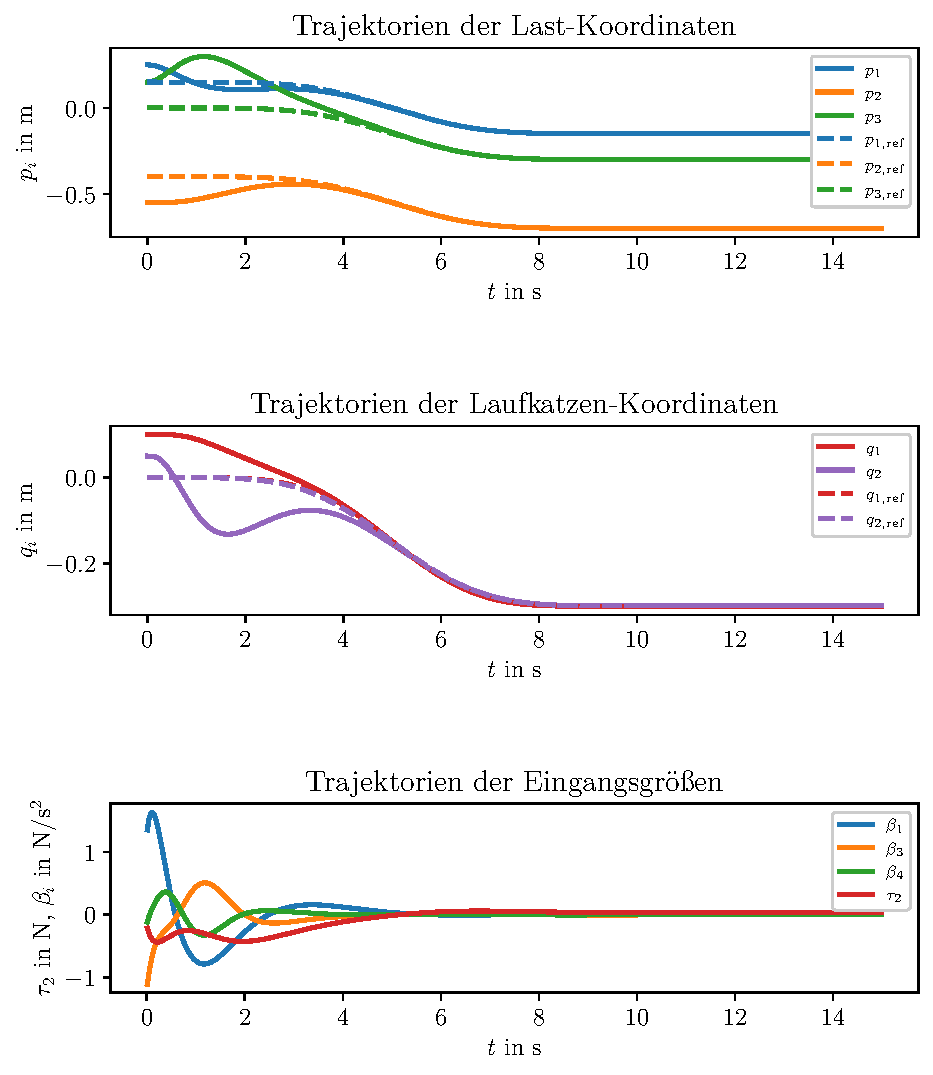
\includegraphics[scale=1]{Pictures/dyn_controller_initial_error}
	\end{center}
	\caption[Kurzbeschreibung für Abbildungsverzeichnis]
	{Langbeschreibung, die gerne auch über mehrer Zeilen gehen darf.}
	\label{fig_dyn_controller_initial_error}
\end{figure}


\subsubsection{Anpassung der Trajektorienplanung}
- an beiden Rändern für jede Referenztrajektorie jeweils 2 mal mehr stetig diffbar wegen weiterer differenzierender Zustände von $\tau_1$, $\tau_3$, $\tau_4$ notwendig -> Trajektorienordnung erhöht sich jeweils um 4

\subsection{Quasi-statische Rückführungen}
Ebenso wie die dynamische Erweiterung kann eine quasi-statische Zustandsrückführung bei einem nicht wohldefiniertem relativen vektoriellen Grad im statischen Ansatz \cite[S. 206]{NLRT_Roebenack}.

\begin{table}[htbp]%
	\centering
	\caption{Auftreten der Eingänge $\tau_j$ bei Ordnung $k$ der Ausgangsableitung $y_i$.}
	\label{tab:relative_degrees}
	\begin{tabular}{ c| c c c c } 
		$k$ & $\tau_1$ & $\tau_2$ & $\tau_3$ & $\tau_4$ \\ 
		\hline
		$y_1^{(k)}$ & 4 & 4 & 2 & 2\\ 
		$y_2^{(k)}$ & 4 & 4 & 2 & 2\\
		$y_3^{(k)}$ & 4 & 4 & 2 & 2\\		
		$y_4^{(k)}$ & 2 & >4 & 2 & 4\\
		$(y_5^{(k)} = q_2^{(k)}$ & >4 & 2 & 4 & 2)\\
		\bottomrule
	\end{tabular}
\end{table}

- Im Folgenden wird der flache Ausgang $\mathbf{y} = (y_1, y_2, y_3, y_4)^T = (p_1, p_2, p_3, q_1)^T$ betrachtet. \\
- Zeitliche Ableitungen werden durch Lie-Ableitungen bezüglich des erweiterten Zustandsvektors $\mathbf{\tilde{x}} = (\mathbf{x}, \mathbf{\tau}, \mathbf{\dot{\tau}})^T$ entlang des Vektorfelds der Zustandsgleichungen $\mathbf{\tilde{\delta}} = \mathbf{\tilde{f}} + \mathbf{\tilde{g}} \mathbf{\tilde{\tau}}$ mit
\begin{align}
\mathbf{\tilde{\delta}} =
\left(\begin{matrix}
\mathbf{f} + \mathbf{g} \mathbf{\tau}\\
\dot{\mathbf{\tau}} \\
\ddot{\mathbf{\tau}}
\end{matrix}\right)
\end{align}

- $\tau_3$ tritt das erste mal bei $r_1 = 2$ in $\ddot{y}_1$ sowie auch in allen anderen zweiten Ableitungen des flachen Ausgangs auf. Dies gilt nicht für alle weiteren Eingänge, da der relative vektorielle Grad für $r_i = 2 \ \forall i$ nicht wohldefiniert ist. \\
- Außerdem tritt $\tau_4$ auch bei $r_3 = 2$ in $\ddot{y}_1$, $\ddot{y}_2$ und $\ddot{y}_3$, nicht aber in $\ddot{y}_4$ auf. \\
-> Widerspruch zu \cite[S. 206]{NLRT_Roebenack}, bei dem für Auftreten von  $u_2$ der Ausgang $y_2$ noch weiter differenziert werden muss! \\ 
- $\tau_2$ tritt erst bei $r_2 = 4$ in $y_1^{(4)}$, $y_2^{(4)}$ oder $y_3^{(4)}$ auf. \\
- $\tau_1$ tritt erst bei $r_4 = 2$ in $\ddot{y}_4$ auf. \\
- Definition neuer Eingänge:
\begin{align}
\begin{split}
	\ddot{y}_1 = \ddot{p}_1 &=: v_1 = \gamma_1(x, \tau_3, \tau_4) \\
	y_2^{(4)} = p_2^{(4)} &=: v_2 = \gamma_2(x, \tau_1, \tau_2, \tau_3, \tau_4, \dot{\tau}_3, \dot{\tau}_4, \ddot{\tau}_3, \ddot{\tau}_4) \\
	\ddot{y}_3 = \ddot{p}_3 &=: v_3 = \gamma_3(x, \tau_3, \tau_4) \\
	\ddot{y}_4 = \ddot{q}_1 &=: v_4 = \gamma_4(x, \tau_1, \tau_3) .
\end{split}
\end{align}

- Daraus ersichtlich, dass aus einem Gleichungssystem aus $v_1$, $v_3$ und $v_4$ in denen alle Eingänge jeweils affin auftreten, eine explizite Darstellung von $\tau_1$, $\tau_3$ und $\tau_4$ möglich ist. \\
-> im Gegensatz zu \cite[S. 207]{NLRT_Roebenack}, bei dem relative Grade der Ausgangskomponenten aufsteigend sind, so dass kein Gleichungssystem gelöst werden muss, sondern sukzessives Einsetzen vorher berechneter Eingänge und Umstellen der abgeleiteten Ausgänge genügt.\\
- Die Berechnung von $\tau_2$ erfordert größeren Aufwand. Dabei Substitution bisheriger Eingangskomponenten und deren Ableitungen, welche aus Lie-Ableitung entlang von $\mathbf{\tilde{\delta}}$ generiert werden. Es folgt ein sehr umfangreicher Ausdruck für $\tau_2$, der bereits zu diesem Zeitpunkt mehr als einhunderttausend Rechenoperationen enthält. \\
- Nach \cite[S. 208]{NLRT_Roebenack} kann eine lineare Fehlerdynamik $\mathbf{v}$ entsprechend jeweiligem relativen Grad der Ausgangskomponente angesetzt werden. Für $v_1$, $v_3$ und $v_4$ diese jeweils nur von Zustandskomponenten abhängig, bei $v_2$ allerdings auch von $\ddot{y}_2 = \ddot{p}_2$ und $y_2^{(3)} = p_2^{(3)}$ :
\begin{align}
	\begin{split}
		\ddot{p}_2 &= L_{\mathbf{\tilde{\delta}}} \dot{y}_2 = L_{\mathbf{\tilde{\delta}}} \dot{p}_2 \\
		p_2^{(3)} &= L_{\mathbf{\tilde{\delta}}} \ddot{p}_2.
	\end{split}
\end{align}

und Ableitungen der anderen Komponenten von $\mathbf{v}$, die wie folgt berechnet werden:
\begin{align}
	\begin{split}
	    \ddot{e} + c_1 \dot{e} + c_0 e &= 0 \\
		e^{(3)} + c_1 \ddot{e} + c_0 \dot{e} &= 0 \\
		e^{(3)} + c_1 (-c_1 \dot{e} - c_0 e) + c_0 \dot{e} &= 0 \\
		e^{(3)} - c_1^2 \dot{e} + c_0 \dot{e} - c_0 c_1 e &= 0 \\
		e^{(3)} + (c_0 - c_1^2) \dot{e} - c_0 c_1 e &= 0 \\
		e^{(4)} + (c_0 - c_1^2) \ddot{e} - c_0 c_1 \dot{e} &= 0 \\
		e^{(4)} + (c_0 - c_1^2) (-c_1 \dot{e} - c_0 e) - c_0 c_1 \dot{e} &= 0 \\
		e^{(4)} + (c_1^3 - 2 c_0 c_1) \dot{e} + (c_0 c_1^2 - c_0^2) e &= 0 \\
		\Rightarrow \text{ für } i = 1,3,4: \dot{v}_i = y_i^{(3)} &= y_{i, \text{ref}}^{(3)} - (c_{i, 0} - c_{i, 1}^2) \dot{e} + c_{i, 0} c_{i, 1} e \\
		\ddot{v}_i = y_i^{(4)} &= y_{i, \text{ref}}^{(4)} - (c_{i, 1}^3 - 2 c_{i, 0} c_{i, 1}) \dot{e} - (c_{i, 0} c_{i, 1}^2 - c_{i, 0}^2) e,
	\end{split}
\end{align}

so dass sich der neue Eingang $v_2$ wie folgt ergibt:
\begin{equation}
	v_2 = y_2^{(4)} = y_{\text{ref}}^{(4)} - c_{2, 3} (y^{(3)} - y_{\text{ref}}^{(3)}) - c_{2, 2} (\ddot{y} - \ddot{y}_{\text{ref}}) - c_{2, 1} (\dot{y} - \dot{y}_{\text{ref}}) - c_{2, 0} (y - y_{\text{ref}})
\end{equation} 

- Problem mit Singularitäten wenn in den Berechneten Stellgrößen wirklich alle gemessenen Zustandskomponenten $\mathbf{x}$ vorkommen statt nur die von $\mathbf{y}$ und seinen Ableitungen.

\subsubsection{Singularitäten in der Nähe von Ruhelagen}
In allen Eingangsgrößen treten bei diesem quasi-statischen Rückführungsentwurf in der Nähe von Ruhelagen Singularitäten auf. Diese ergeben sich aus numerischen Effekten. Beim Einsetzen einer zuvor ermittelten Ruhelage entstehen Definitionslücken, sowohl Zähler als auch Nenner der Eingangsgrößen werden Null. Es ist nicht auszuschließen, dass diese durch algebraische Manipulation hebbar sind. Allerdings ist eine weitere händische Untersuchung dieses Zusammenhangs mit hohem Aufwand verbunden und wird im Rahmen dieser Arbeit nicht weiter verfolgt. Die CAS-Bibliothek SymPy bietet mittels des Aufrufs \texttt{simplify} allerdings keine Lösung dieses Problems in den Eingangsgrößen.

Für eine weitere Betrachtung würden sich die einfacheren Terme der Nenner $N_{1,3,4}$ von $\tau_1$, $\tau_3$ und $\tau_4$ anbieten:
\begin{flalign}
	\begin{split}
	N_{1,3,4} &= s_{2} (- 4 l_{0} pm_{1} \sin{(pm_{3})} + 2 l_{0} pm_{2} \cos{(pm_{3})} + 4 l_{0} qm_{1} \sin{(pm_{3})} + l_{0} s_{2} \sin{(2 pm_{3})}\\
	&+ 4 pm_{1}^{2} \sin{(pm_{3})} - 4 pm_{1} pm_{2} \cos{(pm_{3})}- 4 pm_{1} qm_{1} \sin{(pm_{3})} - 4 pm_{1} qm_{2} \sin{(pm_{3})}\\
	&+ 2 pm_{2} qm_{1} \cos{(pm_{3})} + 2 pm_{2} qm_{2} \cos{(pm_{3})} + 4 qm_{1} qm_{2} \sin{(pm_{3})} - qm_{1} s_{2} \sin{(2 pm_{3})}\\
	&+ qm_{2} s_{2} \sin{(2 pm_{3})}).
	\end{split}
\end{flalign}

Des Weiteren ist die Fragestellung von Interesse, weshalb sich solche Lücken bei der Konstruktion der Trajektorie in den Ruhelagen ergeben.

\subsection{Exact feedforward linearization}
An der Stelle einer Kompensation der Nichtlinearität mittels Rückführung der gemessenen beziehungsweise simulierten Zustandskomponenten wie bei der exakten Eingangs-Ausgangs-Linearisierung wird im Folgenden die Referenztrajektorie eingesetzt. \cite{Hagenmeyer2003}

Heuristisch wird eine Fehlerdynamik der Ordnung zwei für alle Komponenten des Koordinatenvektors angesetzt:
\begin{equation}
	\ddot{\mathbf{\theta}} = \ddot{\mathbf{\theta}}_{\text{ref}} - \mathbf{c}_1^T \dot{\mathbf{e}} - \mathbf{c}_0^T \mathbf{e}.
\end{equation}

Aus der Zusammensetzung des Zustandsvektors $\mathbf{x} = (\mathbf{\theta}, \dot{\mathbf{\theta}})^T$ und der eingangsaffine Zustandsraumdarstellung kann außerdem der Zusammenhang:
\begin{equation}
	\ddot{\mathbf{\theta}} = \mathbf{f}_{[6, 10]}(\mathbf{\theta}) + \mathbf{g}_{[6, 10]}(\mathbf{\theta}) \mathbf{\tau}
\end{equation}

hergestellte werden. Dabei bedeutet die Indizierung $\bullet_{[i, j]}$, die Auswahl der Zeilen $i$ bis $j$ von $\bullet$. Da $\mathbf{\tau} \in \mathbb{R}^4$ und $\mathbf{g}_{[6, 10]} \in \mathbb{R}^{5 \times 4}$ gilt, kann dieser Zusammenhang über die Bildung einer Pseudo-Inversen von $\mathbf{g}_{[6, 10]}^+$ nach dem Eingangsvektor aufgelöst werden:
\begin{equation}
	\mathbf{\tau}= \mathbf{g}^{+}_{[6, 10]} (\mathbf{\theta}) \ (\ddot{\mathbf{\theta}}_{\text{ref}} - \mathbf{c}_{1} \mathbf{\dot{e}} - \mathbf{c}_{0} \mathbf{e} - \mathbf{f}_{[6, 10]}(\mathbf{\theta})).
\end{equation} 

Unter Einsetzen von $\mathbf{\theta}_{\text{ref}}$ in $\mathbf{g}_{[6, 10]}^+$ und $\mathbf{f}_{[6, 10]}(\mathbf{\theta}$ wird die Exact feedforward linearization realisiert:
\begin{equation}
\mathbf{\tau}= \mathbf{g}^{+}_{[6, 10]} (\mathbf{\theta}_{\text{ref}}) \ (\ddot{\mathbf{\theta}}_{\text{ref}} - \mathbf{c}_{1} \mathbf{\dot{e}} - \mathbf{c}_{0} \mathbf{e} - \mathbf{f}_{[6, 10]}(\mathbf{\theta}_{\text{ref}})).
\end{equation} 

\begin{figure}[ht]
	\begin{center}
		% hier keine Skalierung notwendig, wenn Datei schon mit passender figsize angelegt wurde:
		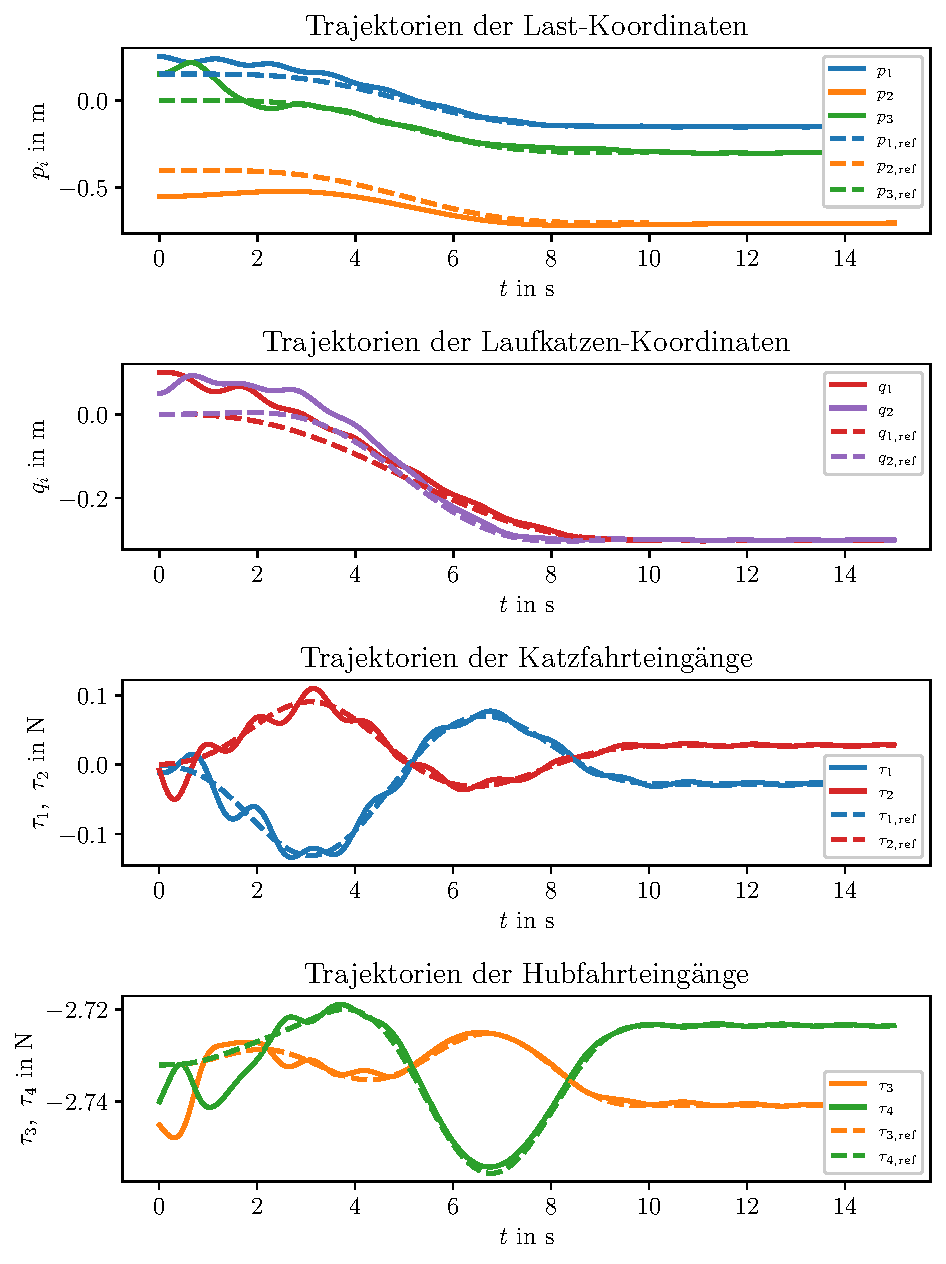
\includegraphics[scale=1]{Pictures/feedforward_lin_pseudo_controller_initial_error}
	\end{center}
	\caption[Kurzbeschreibung für Abbildungsverzeichnis]
	{Langbeschreibung, die gerne auch über mehrer Zeilen gehen darf.}
	\label{fig_feedforward_pseudo_controller_initial_error}
\end{figure}

\subsubsection{Vereinfachung mittels Ausgangsselektion}
Statt der Nutzung einer Pseudo-Inversen kann auch eine Selektion von vier der fünf Gleichungen der Beschleunigungen $\dot{\mathbf{\theta}}$ vorgenommen werden. Symbolisch werde dies über eine Selektionsmatrix $S$ dargestellt:
\begin{equation}
	\mathbf{S} \ddot{\mathbf{\theta}} = \mathbf{S}(\ddot{\mathbf{\theta}}_{\text{ref}} - \mathbf{c}_1^T \dot{\mathbf{e}} - \mathbf{c}_0^T \mathbf{e}) = \mathbf{S} \mathbf{f}_{[6, 10]}(\mathbf{\theta}) + \mathbf{S} \mathbf{g}_{[6, 10]}(\mathbf{\theta}) \mathbf{\tau}.
\end{equation} 

Durch die Wahl der letzten 4 Gleichungen kann eine direkte Inversion der somit quadratischen Eingangsmatrix $\mathbf{g}_{[7, 10]} = \mathbf{S} \mathbf{g}_{[6, 10]}$ erfolgen:
\begin{equation}
	\mathbf{\tau}= \mathbf{g}^{-1}_{[7, 10]}(\mathbf{\theta}_{\text{ref}}) \ \mathbf{S}(\ddot{\mathbf{\theta}}_{\text{ref}} - \mathbf{c}_{1} \mathbf{\dot{e}} - \mathbf{c}_{0} \mathbf{e} - \mathbf{f}_{[6, 10]}(\mathbf{\theta}_{\text{ref}})) \text{ mit } 
	\mathbf{S} = 
	\begin{pmatrix}
	0 & 1 & 0 & 0 & 0 \\
	0 & 0 & 1 & 0 & 0 \\
	0 & 0 & 0 & 1 & 0 \\
	0 & 0 & 0 & 0 & 1 \\
	\end{pmatrix}.
\end{equation}

Diese Berechnungsvorschrift der Stellgrößen enthält deutlich weniger Operationen als alle zuvor dargestellten Ansätze. Damit eignet sie sich insbesondere für eine spätere Implementierung ein Echtzeitsystemen sowie sehr viel kürzeren Simulationszeiten. Es ergibt sich für Beispieltrajektorien mit Anfangsfehlern ein sehr gutes Folgeverhalten sowie eine stationäre Genauigkeit.

\begin{figure}[ht]
	\begin{center}
		% hier keine Skalierung notwendig, wenn Datei schon mit passender figsize angelegt wurde:
		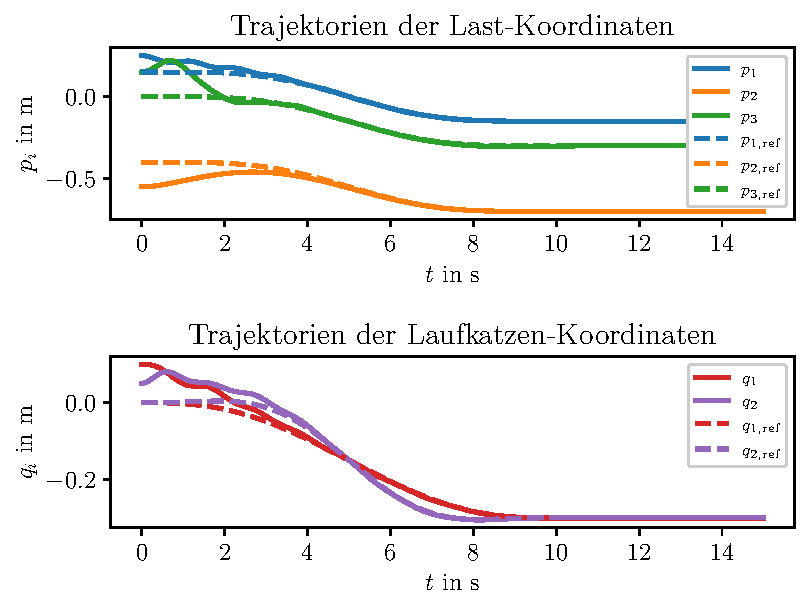
\includegraphics[scale=1]{Pictures/feedforward_lin_selec_controller_initial_error}
	\end{center}
	\caption[Kurzbeschreibung für Abbildungsverzeichnis]
	{Langbeschreibung, die gerne auch über mehrer Zeilen gehen darf.}
	\label{fig_feedforward_selec_controller_initial_error}
\end{figure}

\subsubsection{Stabilitätsbetrachtung}
Die Betrachtung einer prototypischen Trajektorien zeigt, dass zu späteren Zeitpunkten der Simulation Eigenwerte der Jacobimatrix $\mathbf{J}_{\dot{\mathbf{e}}}$ einer Fehlerdynamik:
\begin{align}
	\mathbf{e} := \mathbf{x} - \mathbf{x}_{\mathrm{ref}} \Leftrightarrow \mathbf{x} = \mathbf{e} + \mathbf{x}_{\mathrm{ref}} \\
	\dot{\mathbf{e}} = \dot{\mathbf{x}} - \dot{\mathbf{x}}_{\mathrm{ref}} = \mathbf{f}(\mathbf{e} + \mathbf{x}_{\mathrm{ref}}) + \mathbf{g}(\mathbf{e} + \mathbf{x}_{\mathrm{ref}}) \mathbf{\tau} - \dot{\mathbf{x}}_{\mathrm{ref}} \\
	\mathbf{J}_{\dot{\mathbf{e}}} = \partiell{\dot{\mathbf{e}}}{\mathbf{e}}
\end{align}
mit positiven Realteilen vorkommen. Es ist möglich, dass aufgrund des bis dahin abgeklungenen Folgefehlers keine weitere Destabilisierung des Systems stattfindet, sondern eine stationäre Genauigkeit dennoch erreicht wird. Bis zum Ende der Simulationen weisen alle Eigenwerte erneut einen negativen Realteil auf. Formal kann allerdings bereits am Beispiel einer möglichen Referenztrajektorie mit Ljapunows erster (indirekter) Methode gezeigt werden, dass dieser Regelungsansatz zu einem instabilen System zu gewissen Simulationszeitpunkten führt. Eine andere Wahl von Rückführung (keine lineare Dynamik) könnte dieses Problem lösen.

\begin{figure}[ht]
	\begin{center}
		% hier keine Skalierung notwendig, wenn Datei schon mit passender figsize angelegt wurde:
		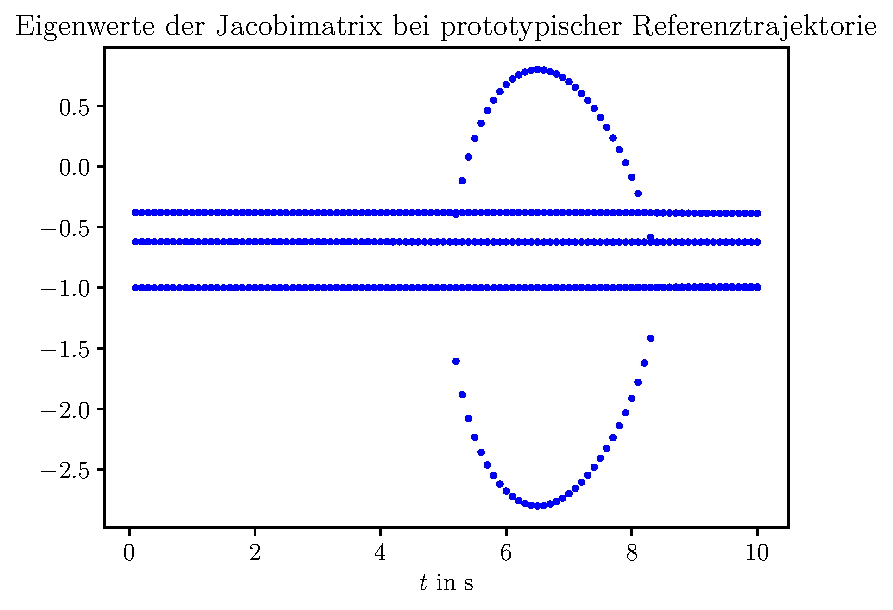
\includegraphics[scale=1]{Pictures/feedforward_lin_selec_ljapunov1}
	\end{center}
	\caption[Kurzbeschreibung für Abbildungsverzeichnis]
	{Langbeschreibung, die gerne auch über mehrer Zeilen gehen darf.}
	\label{fig_feedforward_selec_controller_ljapunov1}
\end{figure}

\chapter{Fazit und Ausblick}
\section{Fazit}
bla

\section{Ausblick}
blub

%%% Local Variables:
%%% mode: latex
%%% TeX-master: "ArbeitRST"
%%% End:
